\chapter{Analysis, Act 1}

\section{Common population models}

Now that we've introduced the idea of stock and flow diagrams, and introduced difference equations, we're going to go on a short tour of some of the common population models. In doing so we will introduce the concept of a 
{\it solution}, 
an {\it initial condition}, and a {\it time-series}.
\subsection{The simplest model of all}

The simplest possible model consists of a single stock, with no flows.  For example, a really simple model of elephants in a game park might look like this:

\centerline{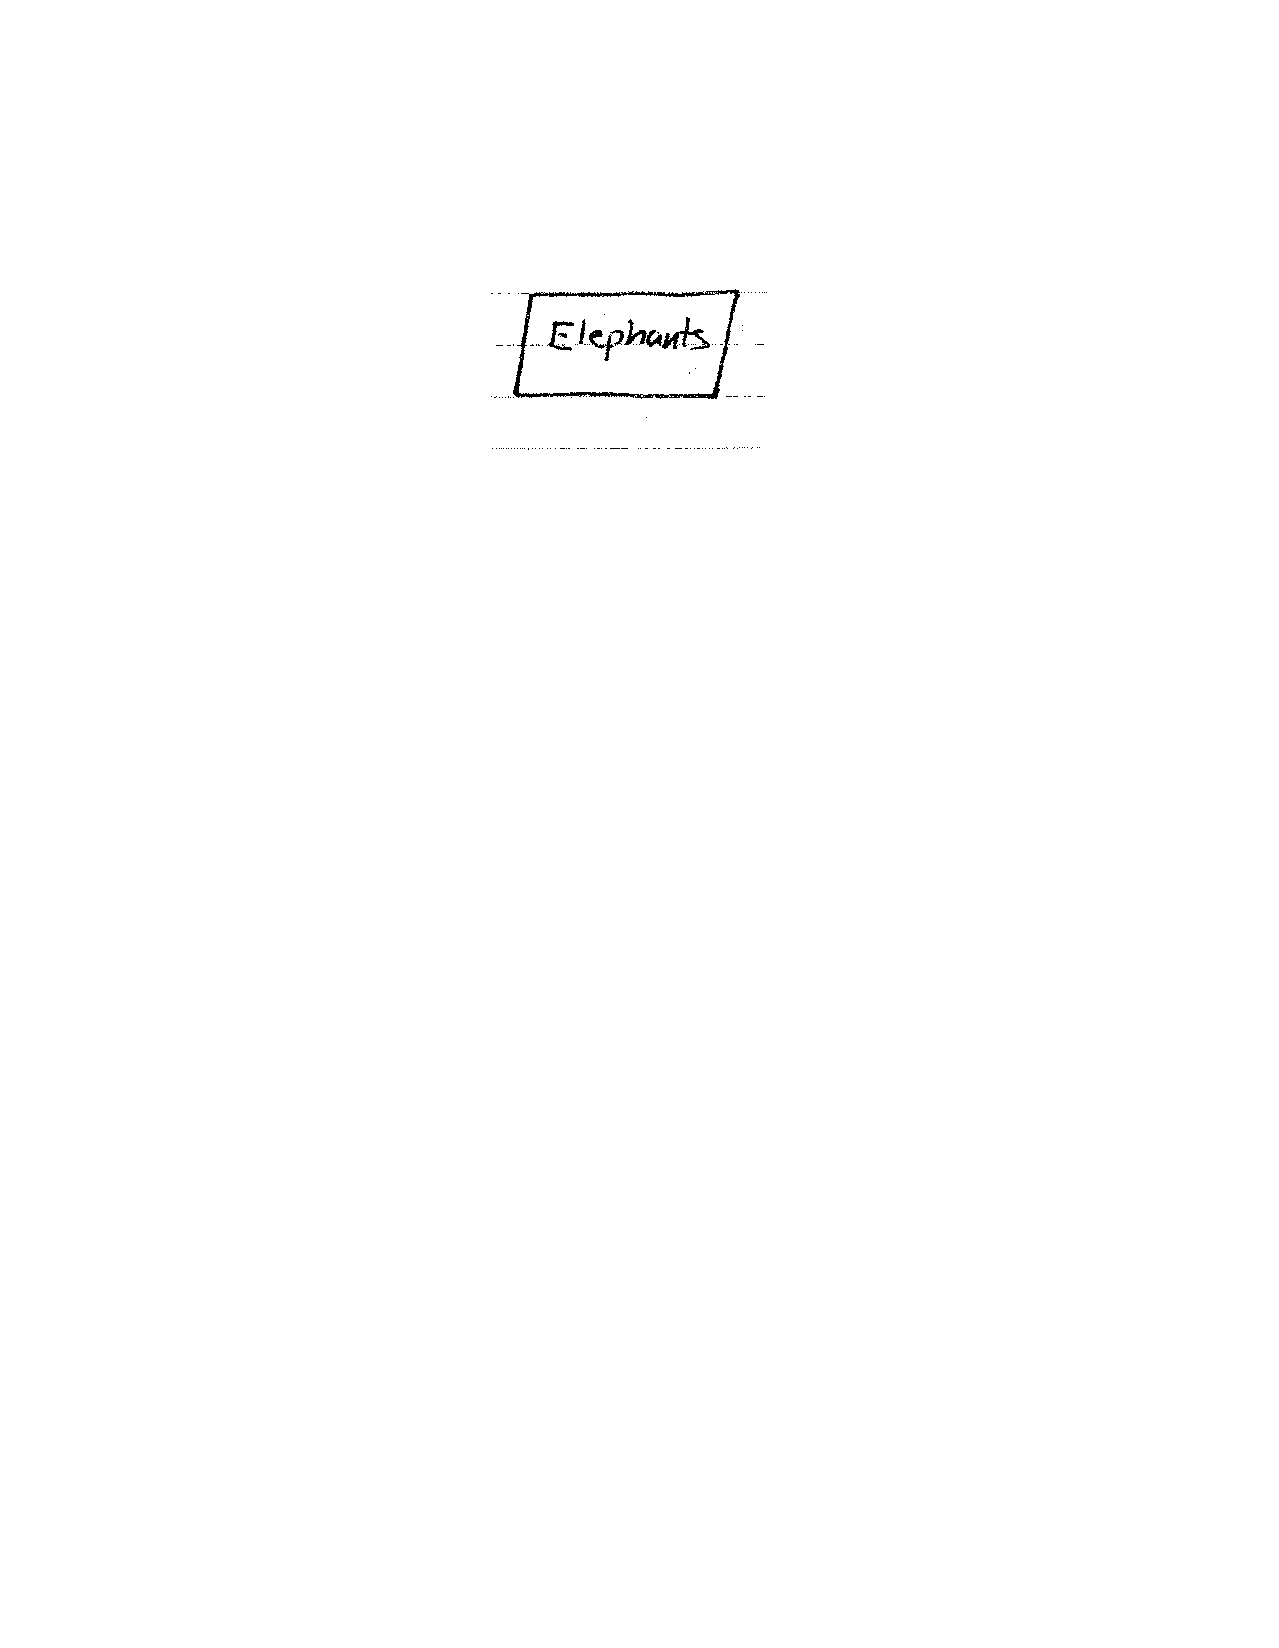
\includegraphics[width=3cm]{figs/simple_model}}

Now, this model is quite strikingly boring, because it says the following:  {\it There are a certain number of elephants in a game park, and there are no processes by which that number of elephants increases or decreases.}  The corresponding difference equation for this model is
\begin{eqnarray*}
E(t+1) = E(t), t = 0, 1, 2, \ldots
\end{eqnarray*}
which has the trivial solution\footnote{A solution is a sequence that satisfies the difference equation and the corresponding initial condition. We will mostly compute solutions by implementing the difference equation in MATLAB, but in some cases it is possible to write down the solution on paper.}
\begin{eqnarray*}
E(t) = E(0), t = 0, 1, 2, \ldots
\end{eqnarray*}
The elephant population is therefore {\bf constant} in time. We might also say that the elephant population is in {\bf equilibrium} as the {\bf net} flow of elephants is zero. Although this model seems ridiculous, in reality it might capture situations in small game parks where dead elephants are immediately replaced and newborn elephants are immediately removed from the park.

\subsection{Zero-order growth}

To make this model a bit more interesting, we might use a zero-order growth model.  Zero-order growth models assume that the number of births, and number of deaths, is independent of the population.  The stock and flow for such a model looks like this:

\centerline{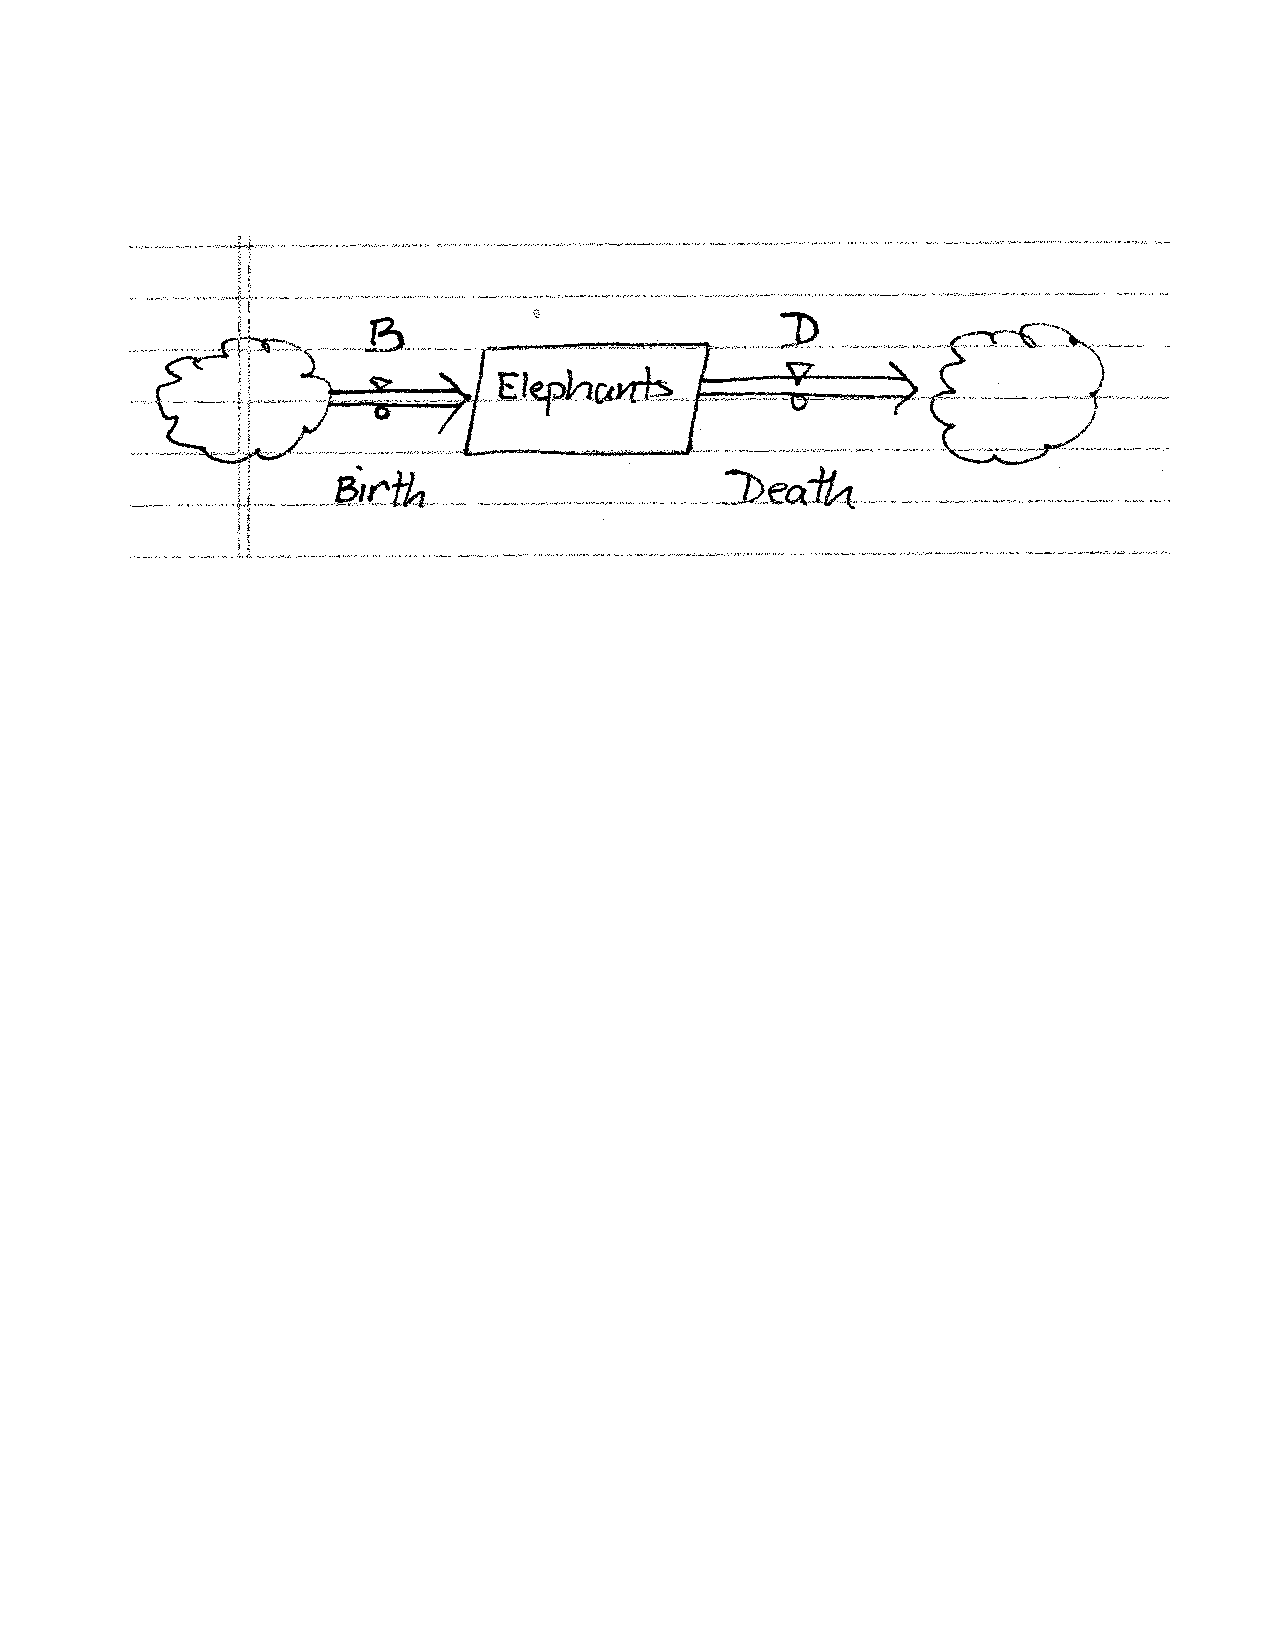
\includegraphics[width=8cm]{figs/zero_order_model}}

The difference equation for a zero-order growth model is then
\begin{eqnarray*}
E(t+1) = E(t) + B - D, t = 0,1,2,\ldots
\end{eqnarray*}
where $B$ and $D$ are the number of births and number of deaths per year respectively. Naturally, this kind of model produces populations that increase or decrease at a constant rate depending on the sign of $B-D$. The solution to this difference equation is
$$ E(t) = E(0) + (B-D)t, t = 0,1,2,\ldots $$
where again $E(0)$ is the initial elephant population. The elephant population is therefore {\bf linear} in time. If $B>D$ the population will increase linearly in time without bound. The time $T_2$ taken by a population to double is often an important quantity, and is given by
$$ T_2 = \frac{E(0)}{B-D}$$
Notice that the time to double in a zero-order model is proportional to the initial population. If $D>B$ the population will decrease and eventually become negative. In Figure 1, we plot the population as a function of time for $B>D$, $B=D$, and $B < D$. This is known as a {\bf time-series} and we will often plot our sequences in this way. Notice that for clarity we plot the discrete data connected by lines. Unless $B=D$ the elephant population can never be in {\bf equilibrium}.

\begin{marginfigure}
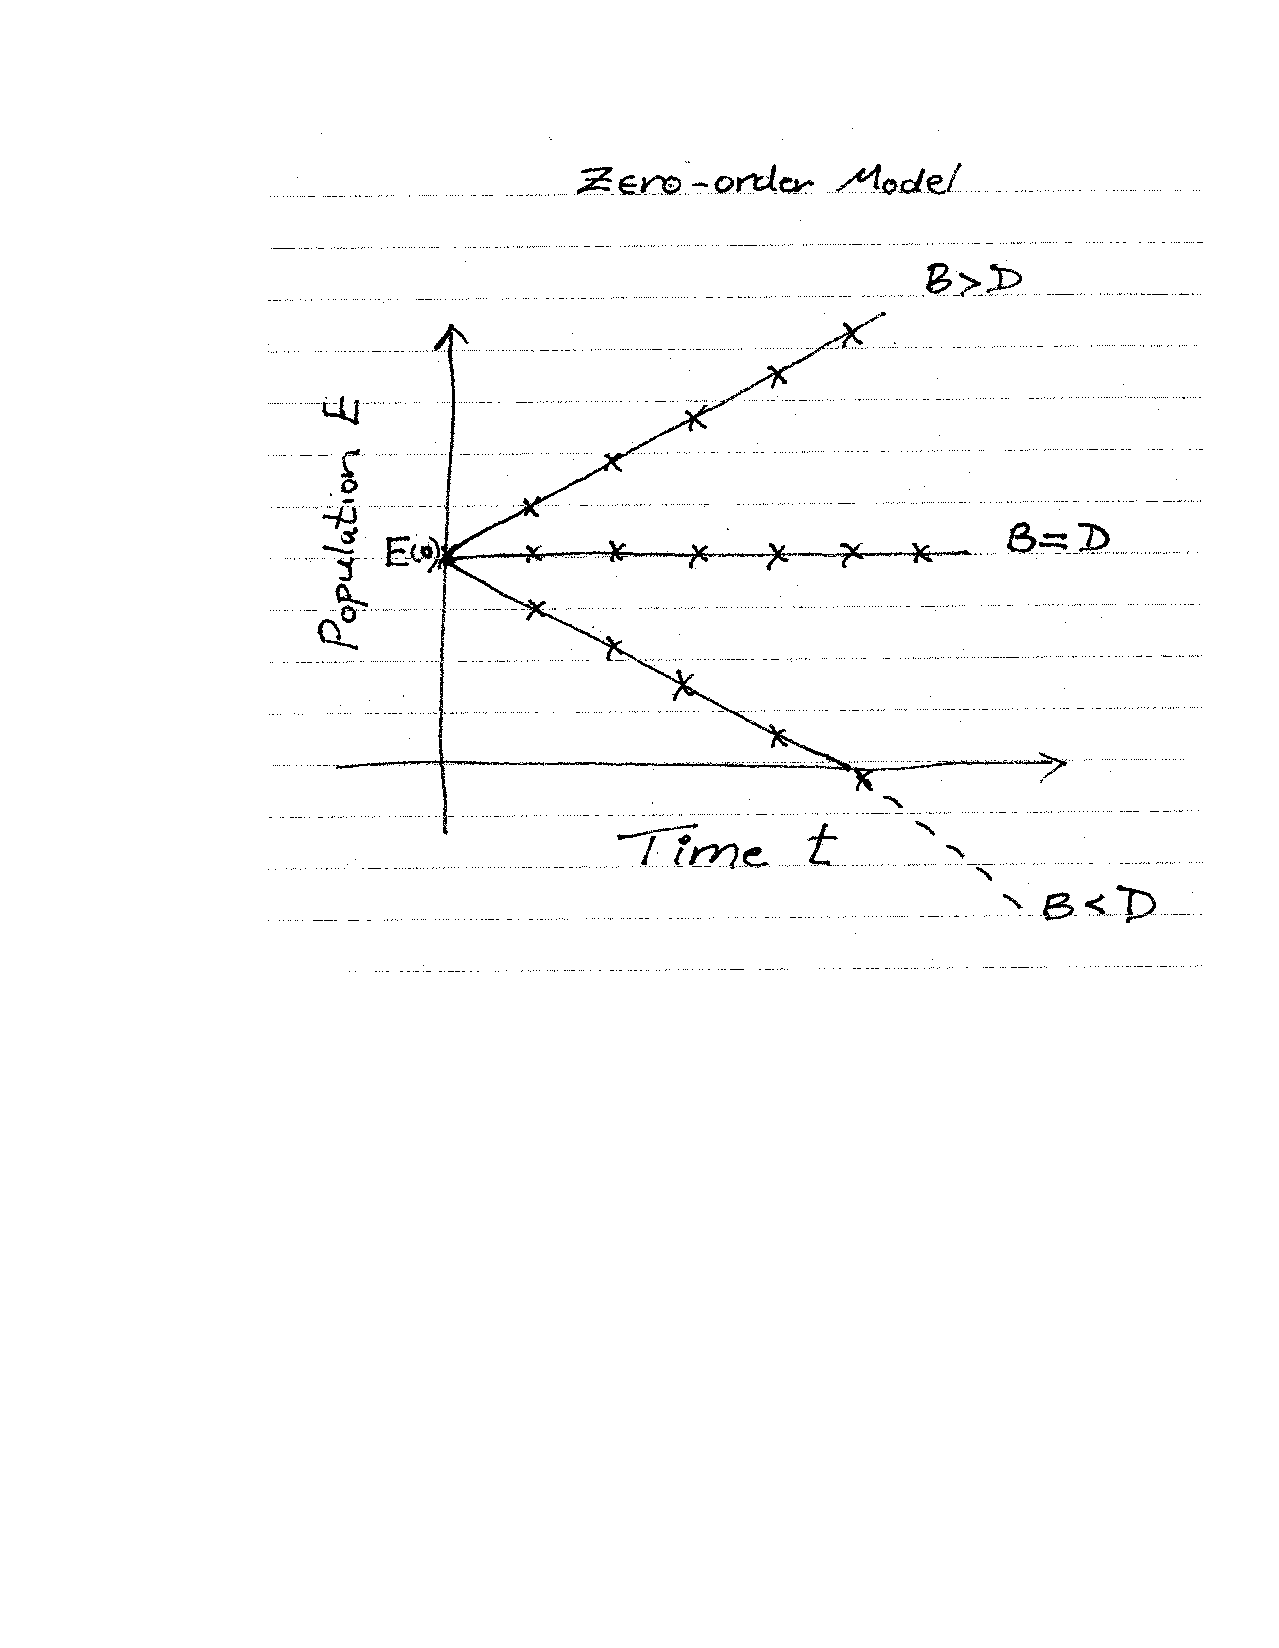
\includegraphics[width=6cm]{figs/zero_order}
\caption{Time-series for zero-order growth models. }
\end{marginfigure}

\begin{del}
How long does it take an initial population of 100 elephants to double if the number of births is 3 elephants per year and the number of deaths is 1 elephant per year? How about an initial population of 1000 elephants? How long would it take the population to halve if the birth and death numbers were reversed?
\end{del}

Neither of these scenarios are realistic over long periods of time, unless the folks in charge of the park practise careful control of the birth and death of elephants. Furthermore, since $B$ and $D$ are independent of $E$, the model suggests that the number of births and the number of deaths is the same regardless of population, which seems rather non-physical too (e.g., 10000 elephants will likely have more babies per year than 100 elephants). However, so long as the model is used in regimes for which is is appropriate -- e.g., for relatively small changes in $E$ -- it can be useful, if not terribly powerful.


\subsection{First-order growth}

A very common population model says that the number of births and the number of deaths each year is proportional to the population:

\centerline{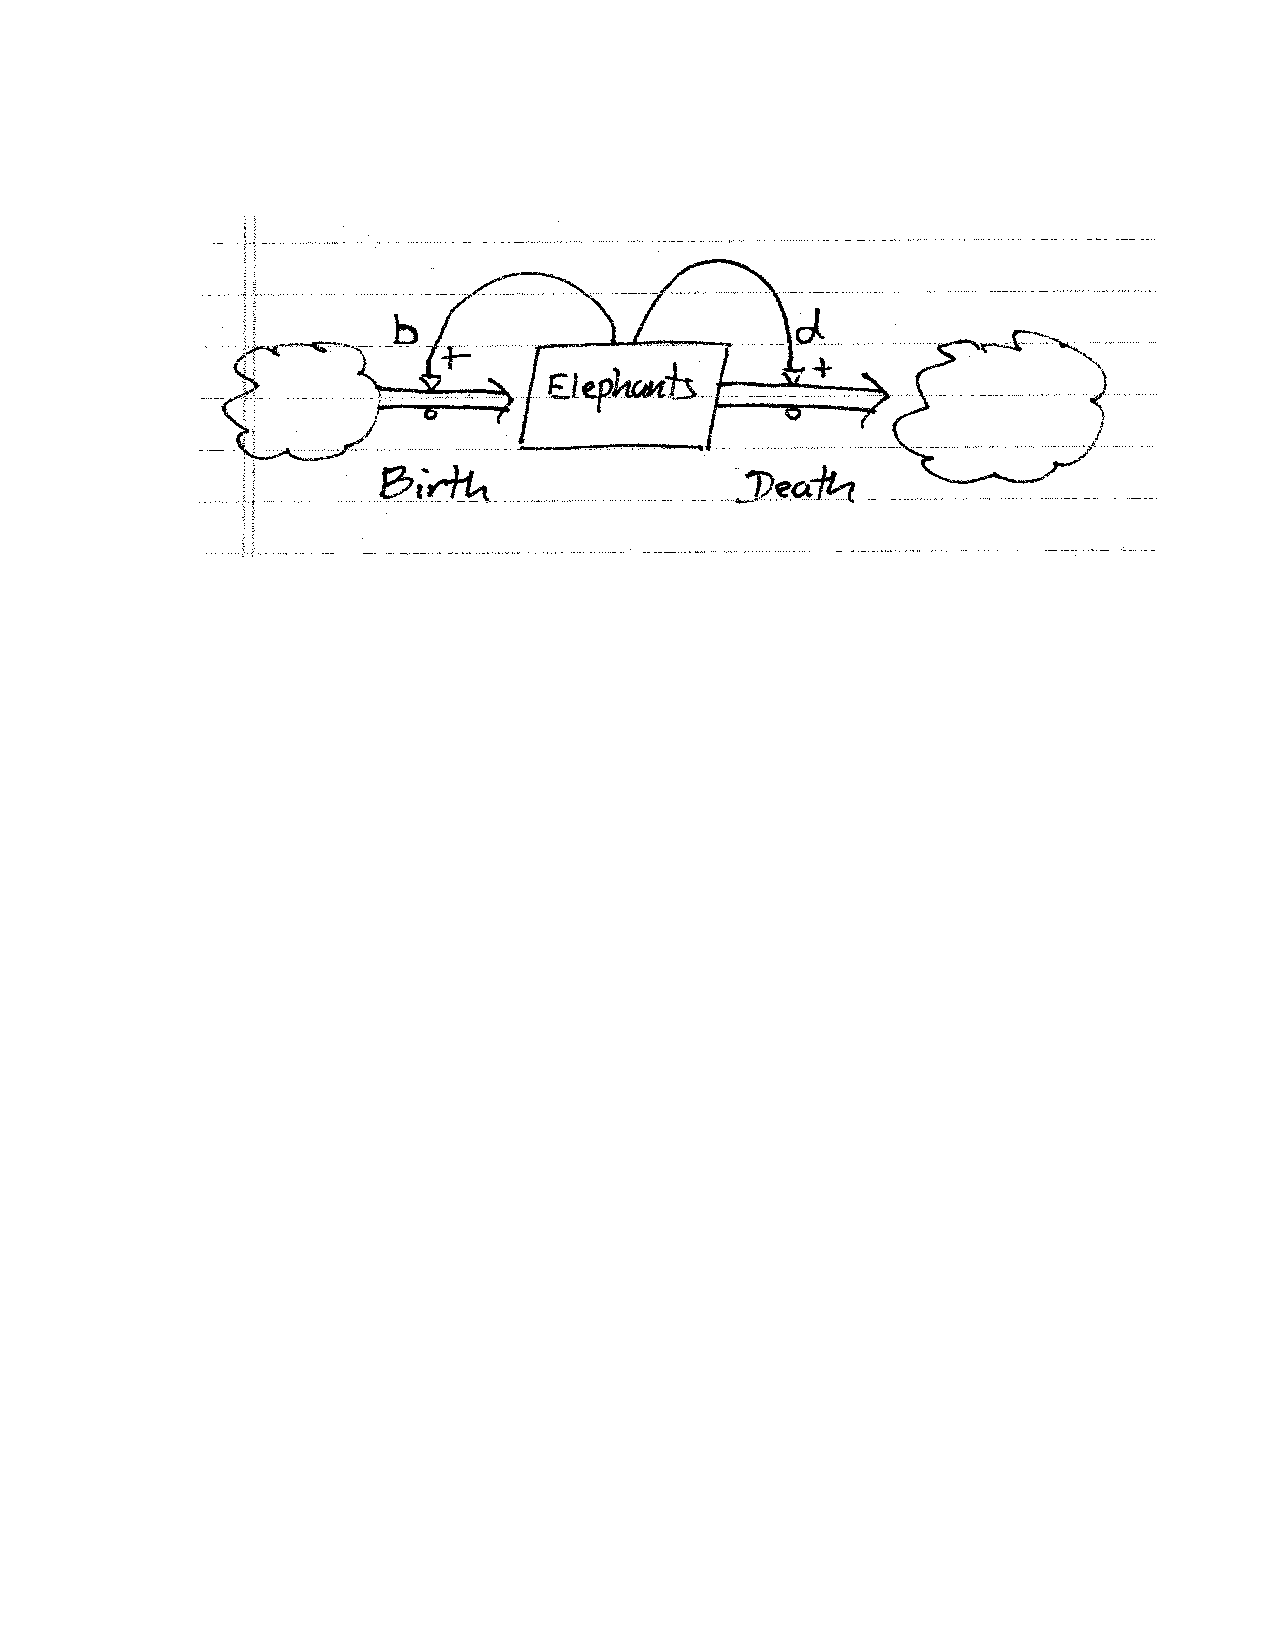
\includegraphics[width=8cm]{figs/first_order_model}}

The difference equation here is
\begin{eqnarray*}
E(t+1) = E(t) + bE(t) - dE(t), t = 0,1,2,\ldots
\end{eqnarray*}
where $b$ and $d$ are the number of births and number of deaths per year per elephant respectively. With appropriate parameters, this kind of model will either give you geometric growth or geometric decay. It's worth asking if there is an elephant population which would be in {\bf equilibrium}. Notice from the difference equation that the change in elephant population from year to year is only zero if the elephant population is zero. While this equilibrium is possible, nothing we have said so far implies that the elephant population will reach this value. In order to find out, let's examine the solution. Again, it is possible to write down the solution to this difference equation on paper
$$E(t) = (1+b-d)^t E(0), t = 0,1,2,\ldots $$
where $E(0)$ is the initial elephant population. This model has slightly more interesting dynamics, depending on the value of $b$ and $d$. Normally you would expect birth and death rates between 0 and 1, which would imply that $0<1+b-d<2$, but let's assume that $b$ and $d$ could take on any value. If $1+b-d > 1$ then the elephant population grows monotonically\footnote{varying in such a way that it either never decreases or never increases.}
. The time $T_2$ taken to double the initial population is now
$$ T_2 = \frac{\ln(2)}{\ln(1+b-d)} $$
which is independent of the initial population. If $0 < 1+b-d < 1$ then the elephant population decays monotonically to zero which is the equilibrium population. If $-1 < 1+b-d<0$ then the elephant population decays to zero while oscillating between positive and negative values and if $1+b-d < -1$ then the elephant population grows while oscillating from positive to negative.

Now if you take a look at the behavior of the population for different values of $1+b-d$, it's pretty clear that some of these regimes, while mathematically interesting, are a bit problematic from a physical perspective.   When $1+b-d<0$, the elephant population {\it oscillates between positive and negative}.  Interesting.  But not very physical.  Why does this happen?  This condition corresponds to $b-d<-1$, so that if the initial population is positive, the net change in the elephant population both negative and {\it larger in magnitude} than the actual population.  In other words, {\it more elephants are dying than exist}.  

This highlights an issue that is important to keep in mind when modeling:  choice of parameters matters enormously.  If you choose non-physical parameter values, the behavior of the model will be non-physical -- no matter how beautiful the equations are.

\begin{marginfigure}
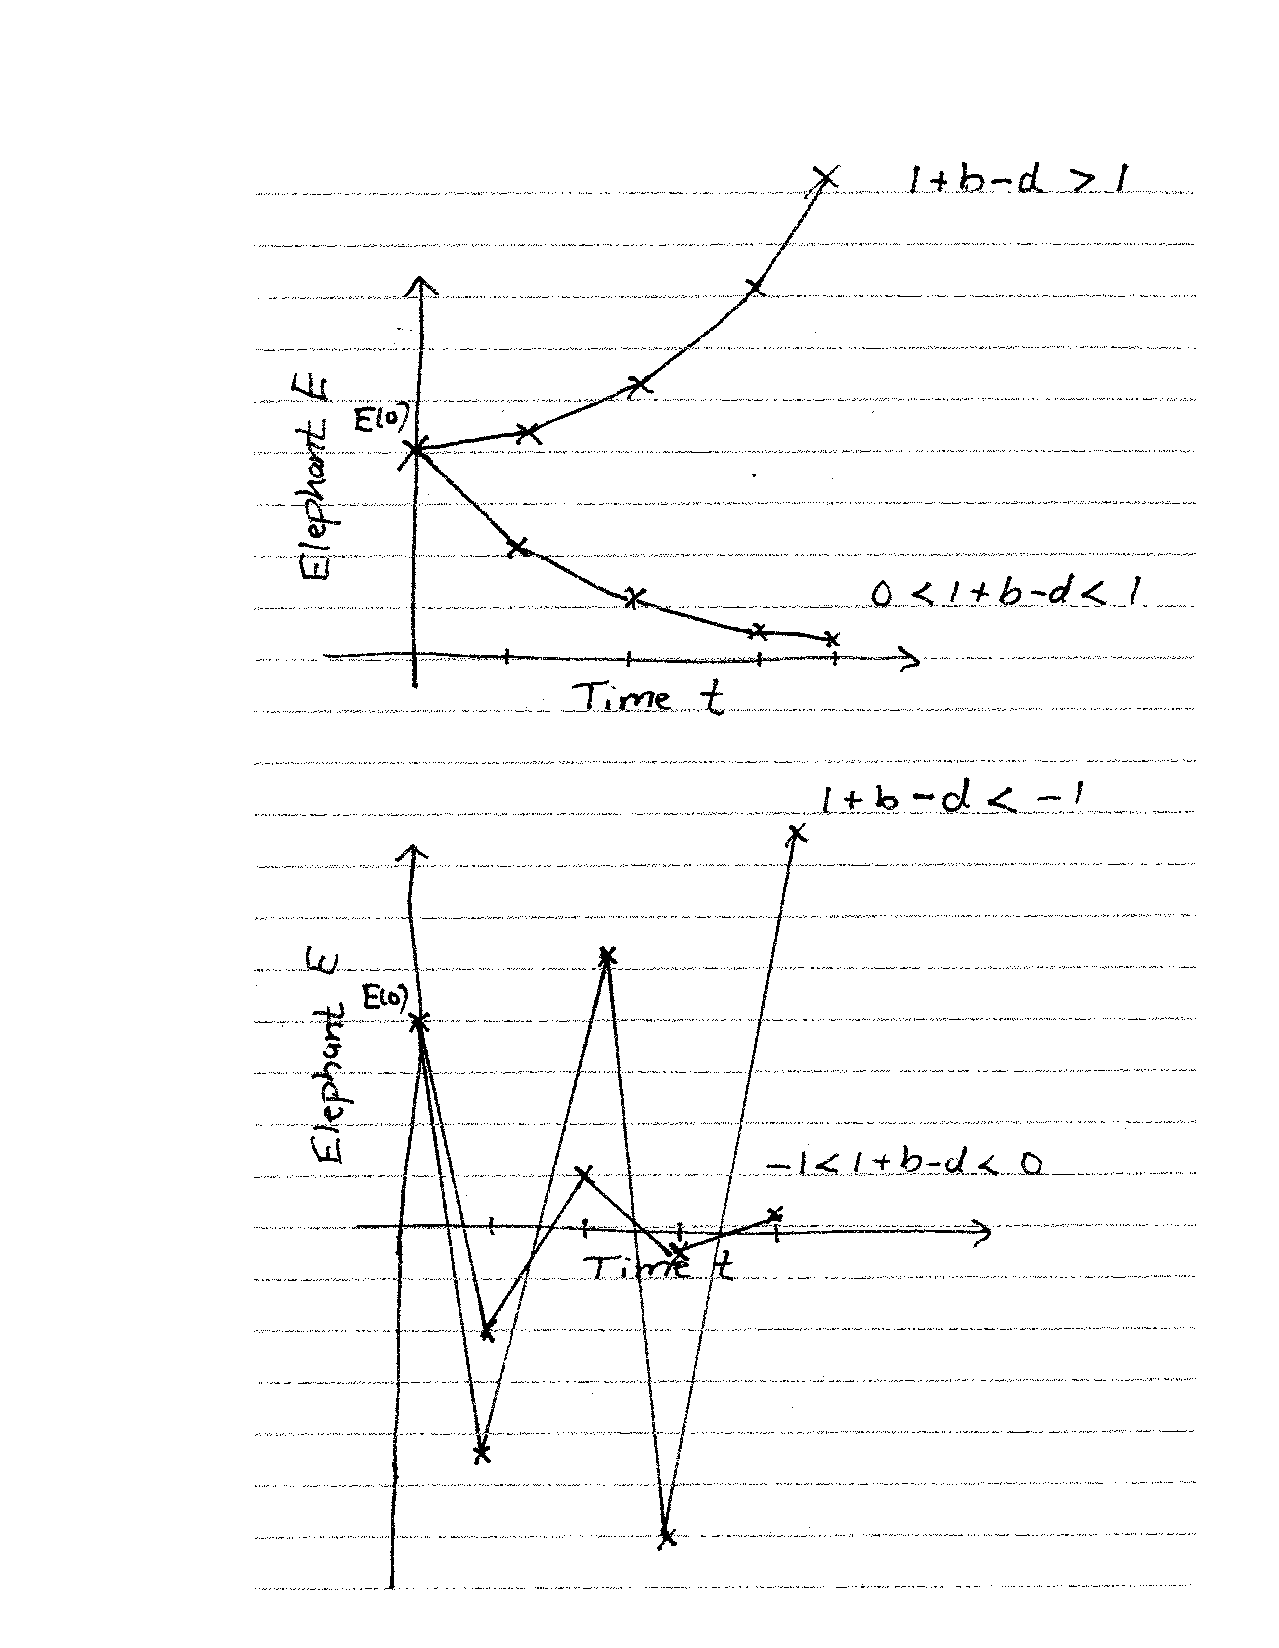
\includegraphics[width=6cm]{figs/first_order}
\caption{Time-series for first-order growth models. }
\end{marginfigure}


\begin{del}
How long does it take the population of elephants to double if the birth rate is 4 \% per year and the death rate is 2 \% per year? How long does it take the population of elephants to halve if the birth and death rates were reversed?
\end{del}

\begin{del}
What is the {\it rule of 72} and how is it related to our current subject?
\end{del}

\subsection{Combined Model}

It's certainly possible to imagine situations in which there is a combination of a zero-order and a first-order model. For example, the following stock and flow diagram has two different types of flow

\centerline{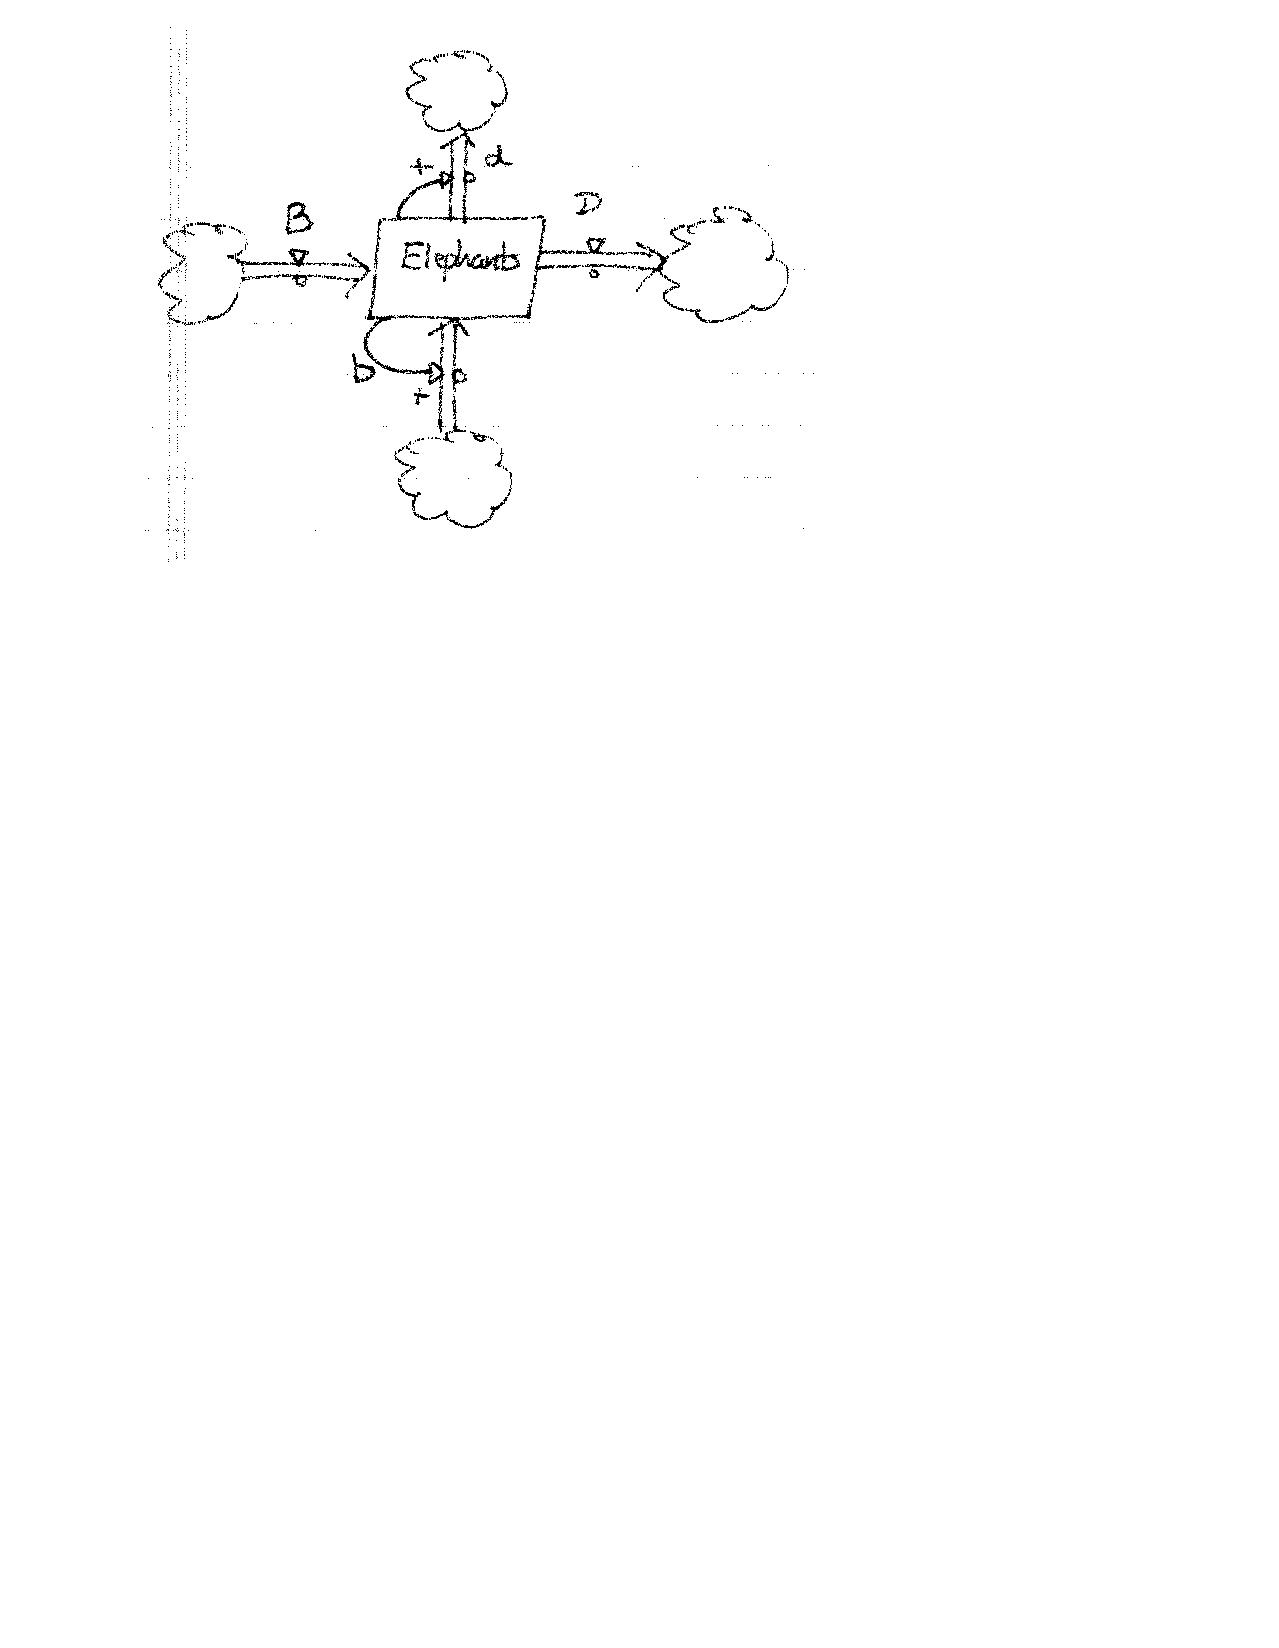
\includegraphics[width=8cm]{figs/combined_model}}

and the difference equation for this model is

\begin{eqnarray*}
E(t+1) = E(t) + (b-d)E(t) + (B-D), t = 0, 1, 2, \ldots
\end{eqnarray*}

At this point we have four parameters. $b$ and $d$ might represent natural birth and death rates, while $B$ and $D$ might represent the number of the elephants added to the park or removed respectively over the course of a year. We've already seen that (and the difference equation shows us) that the values of $b$ and $d$ don't matter per se - rather it is the difference. The same is true for $B-D$. Instead of carrying around 4 parameters, let's combine them and re-write the difference equation as\footnote{Here we are doing some analysis in order to better understand the model and make some basic predictions about the time-series - when you implement this model in MATLAB you might find it easier to keep all of the original parameters.}

\begin{eqnarray*}
E(t+1) = (1+\alpha)E(t) + \beta, t = 0, 1, 2, \ldots
\end{eqnarray*}

where $\alpha = b-d$ is the net birth (or death) rate and $\beta = B-D$ is the net addition (or removal) of elephants. Are there any equilibrium population levels? To find out, we find the elephant population level $E$ which makes the change from year to year zero, i.e.

\begin{eqnarray*}
\alpha E + \beta = 0
\end{eqnarray*}

So $E = -\beta /\alpha$ is an equilibrium population which makes physical sense if either $\alpha$ or $\beta$ is negative but not both. Will the elephant population end up at this equilibrium value in the long-term? Let's find out by finding a solution to the difference equation. Again it is possible to write down a solution on paper, but it's not so trivial, so it might be worth looking at this one in more detail. Let's write out the elephant population from year to year

\begin{eqnarray*}
E(1) &=& (1+\alpha)E(0) + \beta \\
E(2) &=& (1+\alpha)E(1) + \beta = (1+\alpha)^2 E(0) + (1+\alpha)\beta + \beta \\
E(3) &=& (1+\alpha)E(2) + \beta = (1+\alpha)^3 E(0) + (1+\alpha)^2 \beta + (1+\alpha)\beta + \beta 
\end{eqnarray*}

and the general pattern is

\begin{eqnarray*}
E(t) = (1+\alpha)^t E(0) + ((1+\alpha)^{t-1} + (1+\alpha)^{t-2} + \ldots + (1+\alpha) + 1) \beta
\end{eqnarray*}

The term on the right is a geometric series which sums to $\frac{(1+\alpha)^t - 1}{\alpha}$ if $\alpha \ne 0$ otherwise it just sums to $t$. The solution to the combined model is therefore

\begin{eqnarray*}
E(t) = (1+\alpha)^t E(0) + \left\{
\begin{array}{cl}
\frac{(1+\alpha)^t - 1}{\alpha} \beta & \mbox{if} \; \alpha \ne 0 \\
t \beta & \mbox{if} \; \alpha = 0
\end{array}
\right.
\end{eqnarray*}

What exactly does this solution tell us? First of all, it agrees with the solutions we already discussed for the zero-order and first-order growth models: If we set $\alpha=0$ then the solution grows (or decays) linearly in time; if we set $\beta=0$ then the solution grows (or decays) geometrically in time. If $\alpha$ and $\beta$ are both non-zero it's a little easier to interpret if we re-group the terms as

\begin{eqnarray*}
E(t) = (1 + \alpha)^t (E(0) + \frac{\beta}{\alpha}) - \frac{\beta}{\alpha}, t=0,1,2,\ldots
\end{eqnarray*}

So part of the solution grows (or decays) geometrically while part of the solution is constant. If $|1 + \alpha| < 1$ then $E(t)$ will tend towards $-\beta/\alpha$ in the long-run (which was the equilibrium population we found earlier) while if $|1 + \alpha| > 1$ the solution will diverge toward infinity. 

Since for some values of $\alpha$ the population tends towards the equilibrium value, why don't we re-write our difference equation so that it is centered around this value. What on earth does that mean you ask? Instead of keeping track of the number of elephants E, we will keep track of the difference between the number of elephants and the equilibrium value. We will call this new population $e$ and define it as

\begin{eqnarray*}
e(t) = E(t)-(-\beta/\alpha)
\end{eqnarray*}

If you like we have simply redefined what we mean by zero. Replacing this into the original difference equation results in

\begin{eqnarray*}
e(t+1) = (1 + \alpha) e(t)
\end{eqnarray*}

which certainly looks a lot simpler - notice that this is the difference equation for a first-order model and the solution is

\begin{eqnarray*}
e(t) = (1 + \alpha)^t e(0)
\end{eqnarray*}

So, deviations from the equilibrium population value grow or decay geometrically. If $-1 <1+ \alpha < 1$ then the deviation tends toward zero, which means that the original population tends toward the equilibrium value. If $|\alpha| > 1$ the deviation grows without bound.  

\begin{del}
Work through the algebra in this case and make sure you arrive at the same difference equation.
\end{del}

\subsection{Carrying capacity}

Often population models use the idea that a system has some maximum sustainable population -- the so-called ``carrying capacity''.  This is typically implemented as a population-dependent death and/or birth rate:  for populations far below the carrying capacity, the birth and death rates are their ``natural'' unconstrained values; at the carrying capacity, the birth rate minus the death rate is zero (i.e., the population is constant), and above the carrying capacity, the birth rate minus the death rate is negative.

In a stock and flow, such an idea might be represented like this:

\centerline{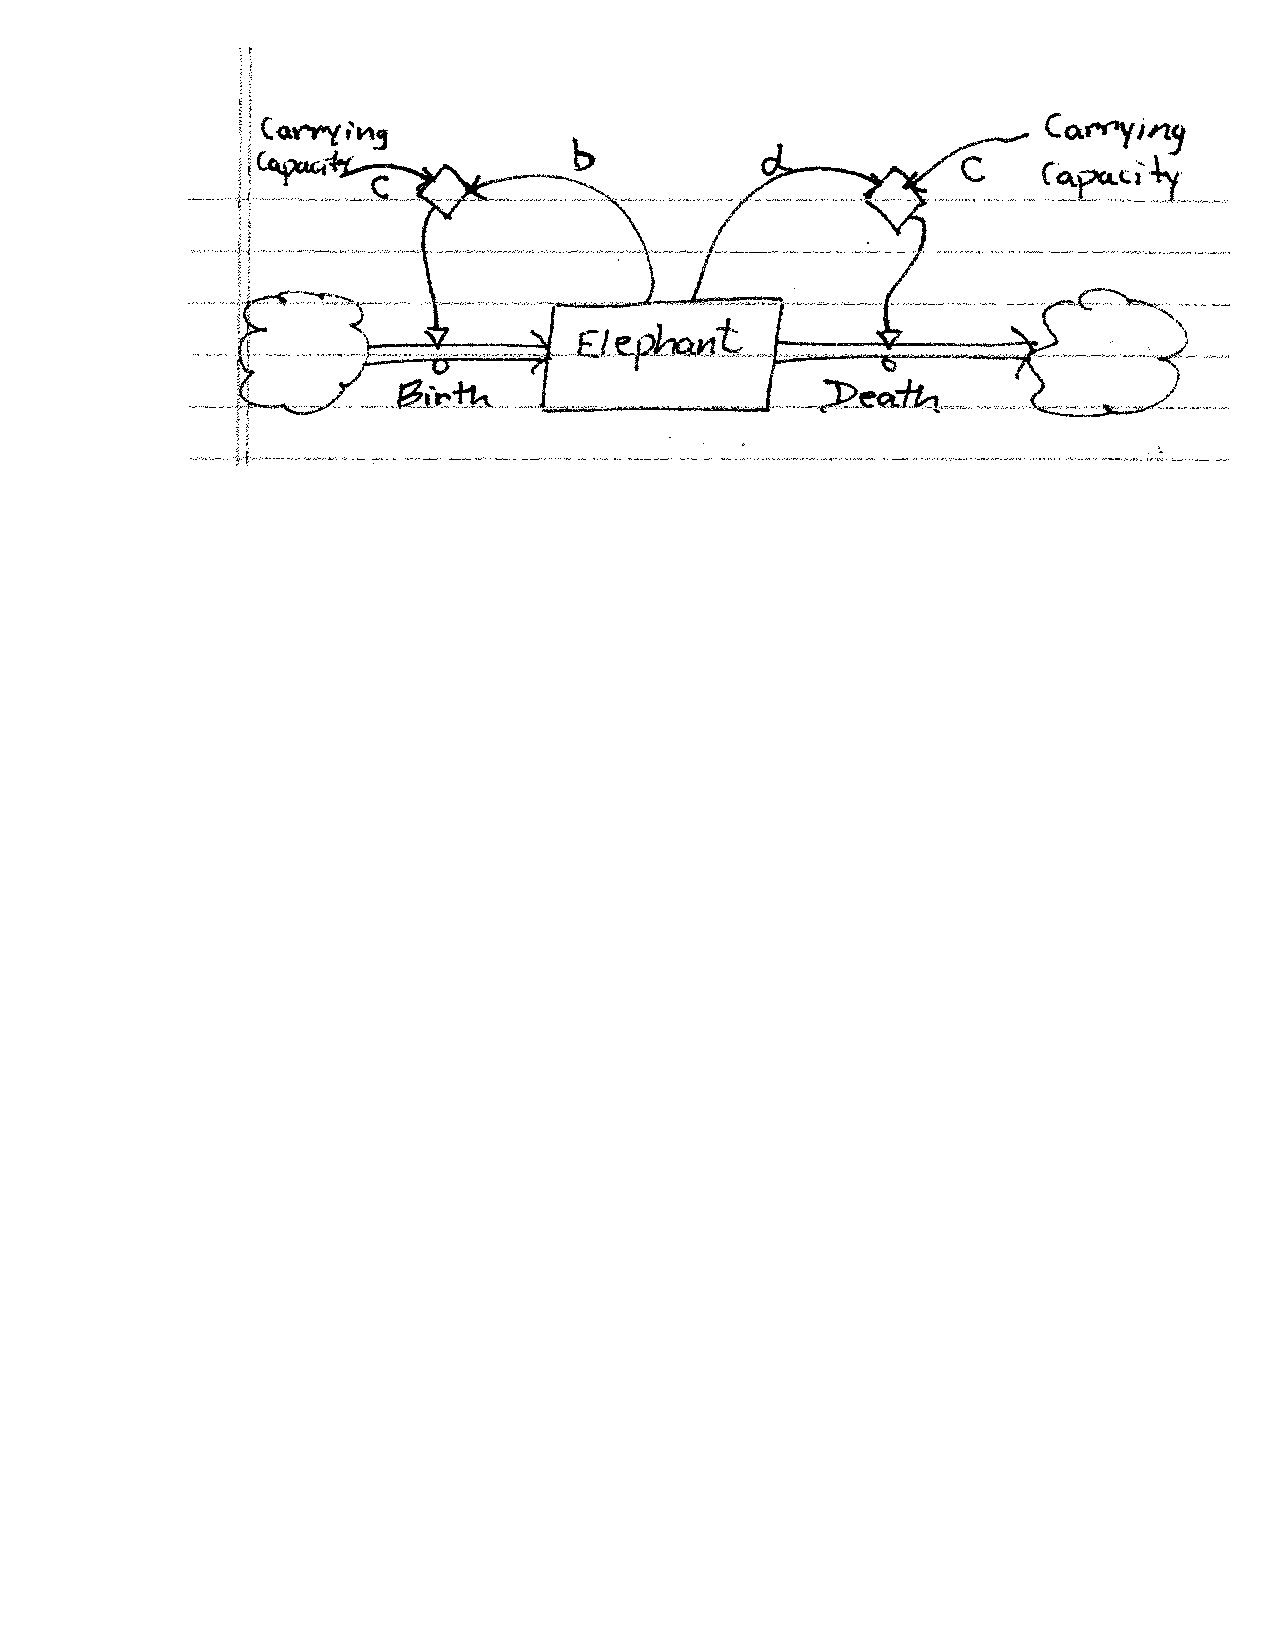
\includegraphics[width=8cm]{figs/carrying_capacity_model}}

Here both death and birth rates depend on the population and on the carrying capacity.  Making this abstraction more concrete, one version of the difference equation might look like this:

$$E(t+1) = E(t) + b(1-\frac{E(t)}{C}) E(t) - d(1+\frac{E(t)}{C})E(t)$$

where $C$ is the carrying capacity of the system.  Note that this equation has the positive feature of correlating directly with the stock and flow:  the birth rate decreases as $E$ gets larger, and the death rate increases as $E$ gets larger.  Of course, if we manipulate this algebraically, we get a simpler equation
 
$$E(t+1) = E(t) + g(1-\frac{E(t)}{C})E(t)$$

where $g = b-d$ is the net growth rate at low populations, and $C$ is the carrying capacity of the system.  Note that when $E=C$, the overall growth rate goes to zero; when $E>C$, the overall growth rate is negative, and when $E<C$, the overall growth rate is positive. Believe it or not, except for a few special cases, the solution to this difference equation cannot be written down on a piece of paper. Indeed the study of this difference equation has resulted in countless Ph.D.'s and is closely connected to the notion of {\bf chaos}. We will return to this a little later, but first let's examine some of the solutions that are possible. 

In Figure 3 we show the time-series for a positive, but small value of $g$. If the initial population is less than the carrying capacity then it will monotonically increase and slowly approach the carrying capacity from below. If the initial population is more than the carrying capacity then it will monotonically decrease and approach the carrying capacity from above. As before, we will refer to the carrying capacity as the equilibrium population - at this population level the birth and death processes are in balance and the net change of population from year to year is zero. 

\begin{marginfigure}
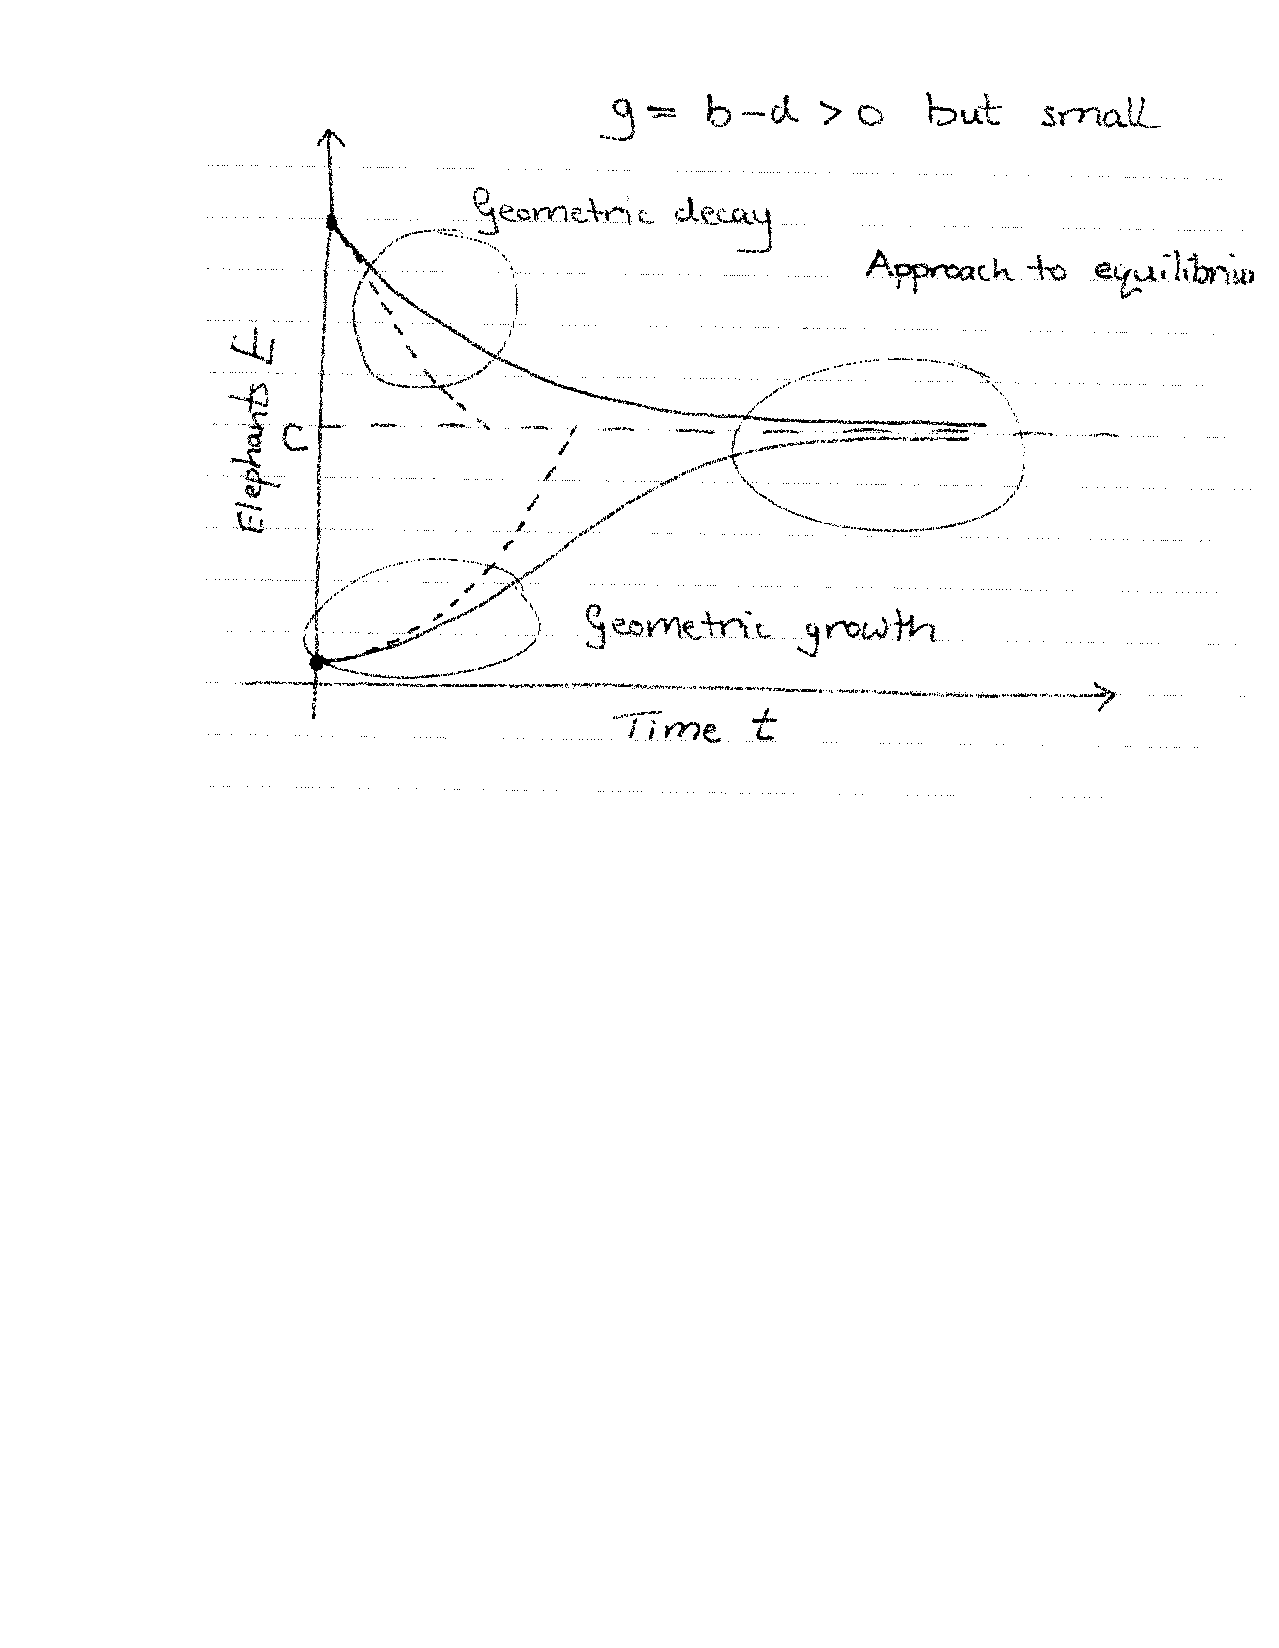
\includegraphics[width=6cm]{figs/carrying_capacity}
\caption{Time-series for model with carrying capacity.}
\end{marginfigure}

The time required for a population to equilibrate is also an important measure which we can estimate. Let's analyse the case where the initial population is small compared to the carrying capacity. In this regime we could approximate the difference equation with

\begin{eqnarray*}
E(t+1) = E(t) + g E(t)
\end{eqnarray*}

because the term involving $gE(t)^2/C$ will be much smaller than $gE(t)$. If we assume that this model is valid then the time to reach carrying capacity would be
\begin{eqnarray*}
T_{C} = \frac{\ln(C/E(0))}{\ln(1+g)}
\end{eqnarray*}
which for $g= 0.02$ and $E(0) = C/10$ would be 116 years. This is certainly an under-estimate of the time to equilibrate because as the population increases the net growth rate decreases, but it gives an order of magnitude.

\begin{del}
Estimate the time required for an initial population $E(0) = 2C$ to equilibrate if $g = 0.02$.
\end{del}  

What if we start with population levels close to the carrying capacity? In this case it makes sense to re-write the difference equation as before and define $e = E-C$. If we replace this into the difference equation we obtain

\begin{eqnarray*}
e(t+1) = e(t) - ge(t) - g \frac{e(t)^2}{C}
\end{eqnarray*}

\begin{del}
Work through the algebra in this case and make sure you arrive at this difference equation.
\end{del}

If we start with a small value of $e$ then the third term will be much smaller than the second term and we can ignore it. The population will then approximately obey the difference equation

\begin{eqnarray*}
e(t+1) = (1-g) e(t)
\end{eqnarray*}

which is another first-order model. If $|1-g| < 1$ then the population will decay geometrically to the carrying capacity. Otherwise it will begin to increase at which point this simplified model breaks down.

\section*{Generalizing Single Stock Population Models}

All of the cases above could be re-written as follows:
$$ E(t+1) = E(t) + \Delta E(E(t))$$
where $\Delta E$ is the change in the population, which depends on what the current population is.


\subsection{Thinking Graphically}
With this formalism, we can compare the models graphically by plotting $\Delta E(E)$.  

\centerline{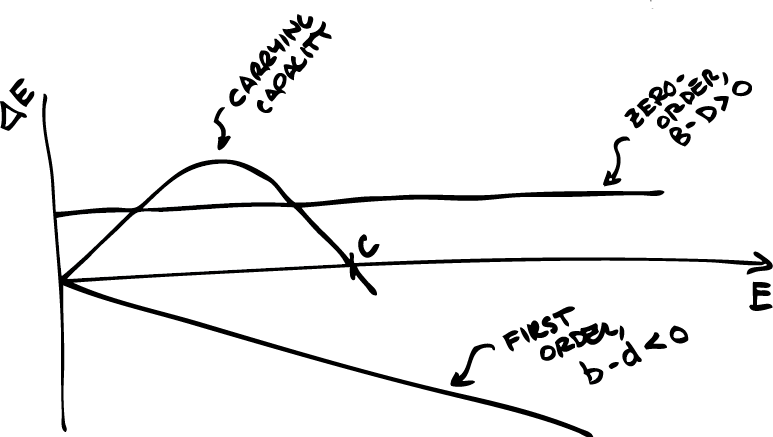
\includegraphics[width=8cm]{figs/DeltaEvsE.png}}

Such a visualization is, in some ways, more useful for explaining the behavior of the model.  For example, in the carrying capacity case, it's easy to see that at small populations the model behaves just like the first order growth model, whereas as the population approaches the carrying capacity, $\Delta E$ approaches zero.  Just as importantly, this visualization can be helpful for {\it building} a model:  it's easy to ask the question, ``How should $\Delta E$ depend on $E$ for small populations?'' than it is to jump immediately to the difference equation.  This kind of visualization becomes more valuable as you start to think about models involving multiple populations, as we will do in a bit.

\subsection{Thinking Analytically}
An alternative approach is to think about the mathematics that underlie the different models we have thus far presented.  In general, we have
$$E(t+1) = E(t) + \Delta E(E(t))$$
So we're interested in how $\Delta E(E)$ behaves.

Pulling out a bit of calculus, we can approximate the behavior of $\Delta E$ in the vicinity of some baseline population $E_0$ using a polynomial (good old Taylor series -- remember those?!):

$$\Delta E(E) \approx c_0 + c_1(E-E_0) + c_2 (E-E_0)^2 + c_3 (E-E_0)^3 + ...$$

where $$c_0 = \Delta E(E_0)$$
 $$c_1 = \frac{d \Delta E(E_0)}{dE} |_{E_0}$$
$$c_2 = \frac{1}{2!}\frac{d^2 \Delta E(E_0)}{dE^2} |_{E_0}$$
 and so forth.

Now, if you take a look at this, you can see that the models we have examined so far (zero-order growth, first-order growth,  and carrying capacity) are in fact simply models that mathematically are equivalent to including the first one, two, and three terms of the Taylor expansion.

In other words, while you can certainly argue for these models from a purely physical perspective (``it makes sense that the number of births/deaths would be proportional to the number of elephants''), you can {\it also} argue for these models from a mathematical perspective (``The simplest possible model involves only the constant term of the Taylor series; the next most complicated involves the linear term as well, and so forth'').  

Since the first few terms in the Taylor series tend to be a good approximation for a function close to the value you are expanding about ($E_0$ above), these approximations should work pretty well {\it so long as we don't get too far away from the baseline population.}  

In short, the canonical models presented above not only make sense from an intuitive, ``yeah, it ought to work that way'' perspective -- they also make sense from a ``keep the math as simple as possible'' perspective.

\section*{Beyond One Stock}

Thus far we've focused on single-stock population models, such as first-order growth and carrying capacity.  These models have the advantage of being relatively simple, and they often admit analysis.  On the other hand, the world is filled with lots of different stocks.  In this section we will introduce a canonical two-stock model:  the Lotka-Volterra predator-prey model.  And we'll also introduce a handy technique for analyzing the behavior of two stock models:  the phase plane.

\subsection*{Lotka-Volterra Predator-Prey}

Imagine a situation in which we have both a predator  species (e.g., foxes) and a prey species (e.g., rabbits).  What model would be appropriate for describing how these two populations evolve in time?

Clearly the population of rabbits matters to the foxes -- if we imagine that rabbits are the primary food supply for foxes, it seems pretty likely that reducing the rabbit population will in turn lead to more fox deaths.  By the same token, increasing the fox population will lead to more rabbit deaths.  So a reasonable guess at a stock-and-flow for this system might look something like this:

\centerline{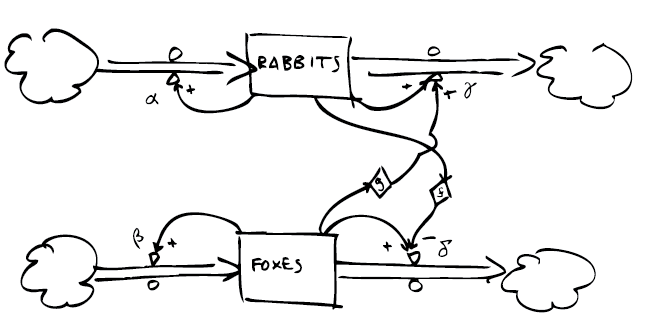
\includegraphics[width=8cm]{figs/RabbitFoxStockAndFlow.png}}

This stock-and-flow is, of course, underdefined -- the death rate functions $f$ and $g$ could be almost anything.

Lotka-Volterra uses the simplest possible version of these functions:  they are simply proportional to the respective populations.  In this case, we get the expressions

$$R(t+1) = R(t) + \alpha R(t) - \gamma F(t) R(t)$$
$$F(t+1) = F(t) + \beta R(t) - \delta R(t) F(t)$$

Mathematically, the expressions above make sense purely from a ``keep the math simple'' perspective.  But if you manipulate the equations a bit, and rename constants,  you obtain:
$$R(t+1) = R(t) + b_r (1 - \frac{F(t)}{F_c}) R(t)$$
$$F(t+1) = F(t) - d_f (1-\frac{R(t)}{R_c}) F(t)$$
These equations are manipulated to allow us to assign meaning to the different terms.  Here $b_r$ is the net rabbit birthrate in the absence of foxes, $d_f$ if the net fox deathrate in the absence of rabbits, $F_c$ is the fox population required to maintain a stable rabbit population, and $R_c$ is the rabbit population necessary to maintain a stable fox population.

Such a mathematical model could be defensible if you make some assumptions:
\begin{enumerate}
\item In the absence of predators (foxes) the rabbit population grows geometrically without bound.
\item In the absence of prey (rabbits), the fox population dies out geometrically.
\item The chance of a given rabbit meeting a fox is proportional to the fox population, and similarly, the chance of a given fox meeting a rabbit is proportional to the rabbit population. 
\end{enumerate}
Note that this last assumption ignores fox-fox competition, and that the first assumption assumes there is an unlimited supply of carrots (infinite carrying capacity).  

\begin{del}
How would the model change if you included fox-fox competition?
\end{del}


\subsection*{Analyzing Predator-Prey: Equilibria and Phase Plane}

With the difference equations in hand  we can analyze the behavior of this system.  One option is to look for equiibria: are there values of $R$ and $F$ such that $R(t+1) = R(t)$, and $F(t+1) = F(t)$?  

\begin{del}
Show that the two equilibria are given by  $\{R=0, F=0\} $, and $\{R=R_c, F=R_c\} $ 
\end{del}

Of course, the more interesting question is what happens if we start with conditions that are {\it not} equilibrium populations.  To analyze this, let's re-invoke the idea of $\Delta E$ that we discussed above.  We'll introduce two terms:

$$\Delta R = b_r (1 - \frac{F}{F_c}) R$$
$$\Delta F= - d_f (1-\frac{R}{R_c}) F$$

So how do these behave?  We will confine ourselves to physically sensible solutions ($R\geq 0$, $F\geq 0$).  Clearly $\Delta R >0$ for $F<F_c$; similarly $\Delta F  > 0$ for $R>R_c$.  So, if we can think about four regions:

\beforefig
\centerline{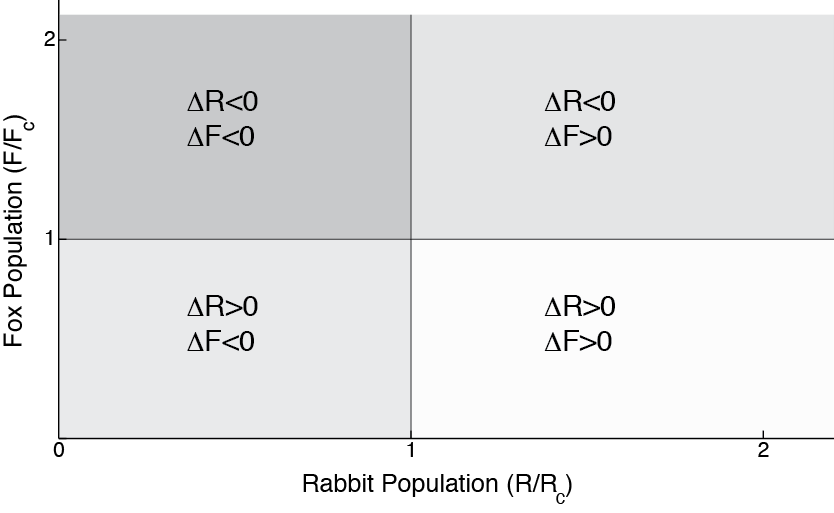
\includegraphics[width=8cm]{figs/FoxRabbitPhasePlaneRegions}}
\afterfig

Starting in the lower left-hand corner, $R<R_c$, and $F<F_c$.  Consequently, foxes are dying ($\Delta F<0$), and rabbits are multiplying ($\Delta R>0$).  As $R$ increases, we reach a region where  $R>R_c$, and $F<F_c$.  This implies that there are now enough rabbits to support foxes, so $\Delta F>0$, while at the same time the number of foxes is too small to suppress increase in the rabbit population, so $\Delta R>0$.  Similar analysis applies to the remaining regions.

A helpful way to visualize the behavior of the system is to use arrows to represent $(\Delta R, \Delta F)$ for a given point.  Such arrows indicate what the populations will be in the following year, if the system starts at the point $R,F$.  With a bit of either hand or computer calculation, it's possible to create a figure that tells us about this (if you're interested in how to do this in MATLAB, read up on {\tt quiver} and {\tt meshgrid}.)

\beforefig
\centerline{
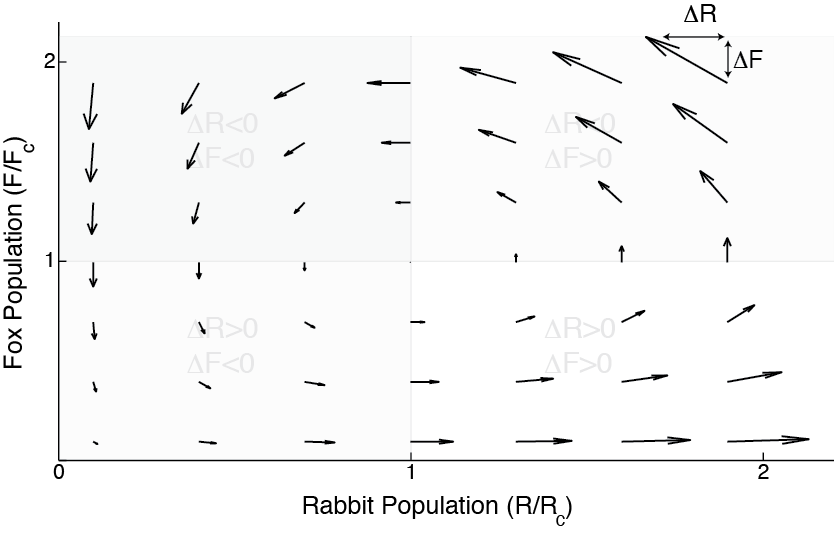
\includegraphics[width=8cm]{figs/FoxRabbitPhasePlaneRegionsWithQuiver.png}}
\afterfig


This plot (which is referred to as the {\it rabbit-fox phase plane} is pretty helpful for seeing how the rabbit and fix populations will evolve in time:  you can imagine ``following the arrows'' to see what the new population is at the end of each year; over time, you would end up traveling in something like a circle:  the rabbit and fox populations appear to be cyclical, and they {\it appear} to oscillate about the equilibrium point -- so the closer to equilibrium you start, the smaller the magnitude of the oscillations.

Note that we've chosen appropriate parameter values for creating this plot.  Just as in the first order growth example above, it's possible to choose very non-physical parameter values for this system -- and get non-physical behavior as a result.


\begin{del}
What values of $b_r$ and $d_f$ are likely to produce non-physical behavior?  Do some analysis on the equations to determine what range of values are likely to ``make sense'' for this system.
\end{del}

At this point we've accrued a fair bit of insight into the behavior of the system, without doing any simulation work.  

\subsection*{Lotka-Volterra Competition Model}

The ideas of the L-V predator-prey model can, of course, be extended to a situation in which you have two species competing for the same food source.  We'll leave it as an exercise for you to think through this (with help, of course, from the wonders of the interwebs).


\section*{Some Interesting Mathematics: The Logistic Difference Equation}

As mentioned earlier, the difference equation for a population model with carrying capacity has received a lot of attention over the years. It was popularised in 1976 by Robert M. May \footnote{Simple Mathematical Models with Very Complicated Dynamics, Robert M. May, Nature 261, 1976.} in the journal Nature as a simple mathematical model for population dynamics which exhibited extraordinary behaviour. This fascinating and highly readable review paper explains the dynamics of difference equations using the logistic difference equation,
\begin{eqnarray}
x(t+1) = \lambda x(t) (1 - x(t)), t = 0, 1, 2, \ldots
\end{eqnarray}
as its chief example. The author goes on to argue that
\begin{quote}
I would therefore urge that people be introduced to [the logistic difference equation] early in their mathematical education.
\end{quote}
I'm afraid to say that, as far as I can tell, this plea has fallen on deaf ears.

We saw earlier that a common population model including carrying capacity results in the difference equation
\begin{eqnarray*}
E(t+1) = E(t) + g(1 - \frac{E(t)}{C}) E(t)
\end{eqnarray*}
where $E(t)$ is the population of elephants in year $t$, $g$ is the net growth rate at low populations, and $C$ is the carrying capacity. At first glance, this model looks similar to the logistic difference equation but not identical - after all it has two parameters and the terms are a little different. However, with a suitable change of variables we can turn this population model into the logistic difference equation discussed by May. If we scale the elephant population and define a new variable
\begin{eqnarray*}
x(t) = \frac{g}{C(1+g)} E(t)
\end{eqnarray*}
and substitute this into the population model then we obtain
\begin{eqnarray*}
x(t+1) = (1+g) x(t) (1-x(t))
\end{eqnarray*}
which is precisely the logistic difference equation if we define $\lambda = 1 + g$. Since $g$ is the net growth rate at low populations we would expect $1+g$ to be close to $1$. However, for the sake of mathematical exploration, we will investigate the logistic difference equation for all values of $\lambda$.
 
\subsection*{Numerical Iteration}

The logistic difference equation,
\begin{eqnarray}
x(t+1) = \lambda x(t) (1-x(t)),
\end{eqnarray}
depends on a single {\bf control parameter} $\lambda$. We will investigate the dynamics of the logistic difference equation by choosing a value for $\lambda$, a value for the initial condition $x(0)$, and then use the difference equation to compute the next few  iterates,
\begin{eqnarray*}
x(1) &=& \lambda x(0) (1-x(0)), \\
x(2) &=& \lambda x(1) (1 - x(1)), \\
\ldots &=& \ldots.
\end{eqnarray*}
For example, let's choose $\lambda = 2$ and $x(0) =\frac{1}{4}$. The next iterate $x(1)$ is
\begin{align*}
x(1) &= (2) (\frac{1}{4})  (1 - \frac{1}{4}), \\
\Rightarrow x(1) &= \frac{3}{8}.
\end{align*} 

\begin{del}
Compute the next 5 iterates by hand using exact arithmetic. What happens to the sequence?
\end{del}

While we can certainly continue this by hand, this is a perfect job for a computer.

\begin{del}
Write a MATLAB script to compute the first 40 iterates of the logistic difference equation for $\lambda = 0.5, 2, 3.2, 3.83, 3.9$, and $4.1$ using the same initial condition $x(0) = 0.25$ in each case.
\end{del}

For reference you should find the following. At $\lambda = 0.5$ the sequence converges rapidly to zero. At $\lambda=2$ the sequence converges fairly quickly to a value that doesn't change. For $\lambda=3.2$ the sequence doesn't converge to a single value but rather oscillates between two different values. For $\lambda=3.83$ the sequence oscillates again, but this time between three different values. For $\lambda=3.9$ the sequence shows no discernible pattern. Finally at $\lambda = 4.1$ the sequence diverges toward $- \infty$.

\subsection*{Long-term behaviour}

\begin{figure}[h]
\centering
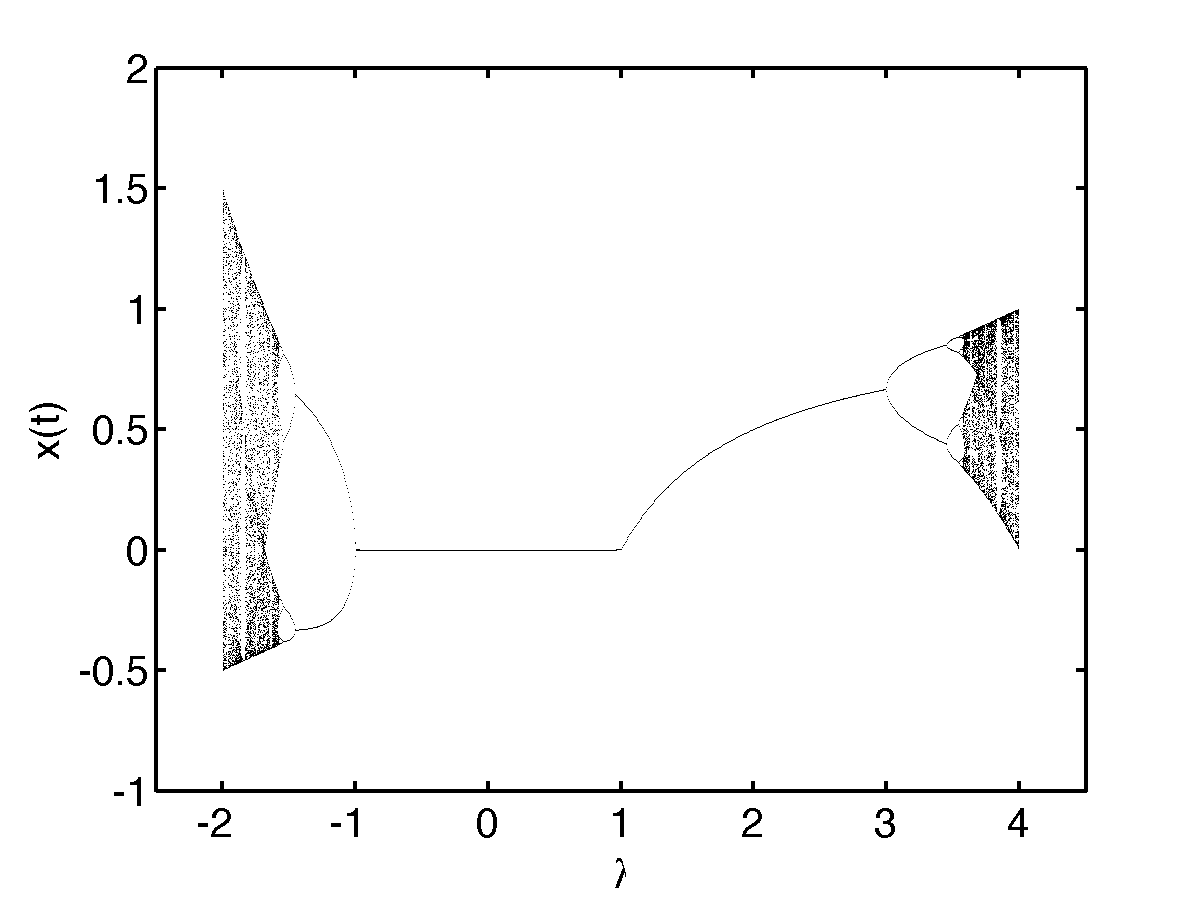
\includegraphics[width=10cm]{figs/logistic_orbit}
\caption{Orbit diagram of the logistic map with $x(0) = 0.25$.}
\label{figure.logistic_orbit}
\end{figure}

One method of visualising the long-term behaviour of the solution is to generate an orbit diagram in which we vary the value of the control parameter and plot the members of the orbit after transients (this is also known as a bifurcation diagram in the literature).  For example, we compute 1000 iterations of the logistic map for different values of $\lambda \in [-2.5,4.5]$ using $x(0) = 0.25$ and we plot the last 100 iterations in Figure (\ref{figure.logistic_orbit}) for each value of $\lambda$. 

There is nothing magical about 100 and 1000 and the number of values of $\lambda$ - we want enough iterations (in this case 1000) so that the sequence settles down but we don't want to keep too many (in this case 100) as it may make the resulting plot very confusing and slow to draw. We want enough {\bf resolution} in $\lambda$ so that we don't miss anything. This diagram succinctly captures the long-term behaviour of the difference equation for a range of values of $\lambda$. For example, for $\lambda \in [-1,1]$ it demonstrates that the orbit converges to zero (at least with the initial condition of $0.25$). For $\lambda$ slightly greater than three, the orbit diagram has two values corresponding to the two values of the periodic orbit. For $\lambda$ close to four there is a dizzying set of points with incredible structure which you will explore. Note that for $\lambda < -2$ and $\lambda > 4$ the orbit diverges rapidly and thus no points appear in this regime.

\begin{del}
Write a MATLAB script to plot the orbit diagram for the logistic difference equation. Carefully generate and explore this diagram for $\lambda \in [3,4]$ and catalogue some of your findings. 
\end{del}

Recall that the logistic difference equation is equivalent to our carrying capacity model with $\lambda = 1+g$ and $x = gE/C(1+g)$. For small positive or negative values of $g$ the orbit diagram agrees with our earlier findings. If $g$ is positive but small the population converges to a single non-zero value (the carrying capacity). If $g$ is negative but small the population converges to zero. The orbit diagram reveals what happens if we make $g$ large. For example, at $g=2$, the equilibrium destabilises and the population settles into an oscillation between 2 different values. Increasing $g$ leads to an oscillation between 4 values, and then 8 values, and then at $g=3.57$ all hell breaks lose and the population begins to fluctuate erratically form year to year - indeed it is {\b chaotic}. Increasing $g$ further results in more chaotic oscillations interspersed with windows where the population oscillates regularly. For $g$ greater than 3 the population diverges to $-\infty$. Similar behaviour occurs when $g$ is made more negative.  In some sense this isn't surprising - after all a net growth rate in excess of $200 \%$ is outrageous. What is surprising (at least to mathematicians) is that the dynamics exhibited by the logistic difference equation appear to be universal, i.e. they are shared by many other difference equations.
%
%\end{document}
%
%
%\section*{Bounded versus Unbounded Orbits}
%We've already seen from the orbit diagram that some orbits are bounded while others are unbounded. For example, with an initial condition of $x(0)=0.25$, {\bf all} of the orbits for $\lambda \in [-2,4]$ are bounded, while {\bf almost all} of the orbits for $\lambda$ outside of this interval are unbounded (for some values of $\lambda$ the initial condition $x(0)=0.25$ is eventually mapped to a fixed-point or periodic orbit). This leads us to make the following conjecture
%
%\begin{con}
%Assume $\lambda \in [0,4]$. If $x(0) \in [0,1]$ then all of the orbits are bounded in $[0,1]$, otherwise the orbits diverge to $-\infty$.
%\end{con}
%
%We will appeal to the cobweb diagram to accept or reject this statement. The case of $\lambda = 0$ is straight-forward since every initial condition gets mapped to zero. For $\lambda > 0$ the logistic map defines a parabola that opens down and is pinned to the origin at $x=0$ and $x=1$. The maximum value (which occurs at $x=0.5$) of the parabola is $\lambda/4$ which is less than or equal to one if $\lambda \leq 4$. Therefore, any initial condition $x(0) \in [0,1]$ will be mapped to $x(1) \in [0,1]$ which will be mapped to $x(2) \in [0,1]$ and so forth producing a bounded orbit in $[0,1]$. On the other hand, any initial condition $x(0) < 0$ will be mapped to $x(1) < x(0) < 0$ which will be mapped to $x(2) < x(1) < x(0) < 0$ and so forth diverging to $-\infty$. Initial conditions $x(0) > 1$ will be mapped to $x(1) < 0$ which will then get mapped to $-\infty$. 
% 
%\begin{del}
%What happens if $\lambda > 4$? $\lambda < 0$? Can you make a conjecture about the long-term behavior of the orbits, and use cobweb diagrams to accept or reject?
%\end{del}
%
%\begin{del}
%Can you make a similar conjecture about the Ricker map and use cobweb diagrams to accept or reject?
%\end{del}
%
%\section*{Fixed-Points}
%We've seen that for some values of the control parameter the orbits of the logistic map converge to a single value known as a fixed-point. Fixed points of any iterated map are defined as those points $x^*$ which are mapped to themselves after one iteration, i.e.
%\begin{eqnarray*}
%x^* = f(x^*)
%\end{eqnarray*}
%For example, $x^*=0$ is always (for any value of $\lambda$) a fixed-point of the logistic map because $f(0) = 0$. In addition, $x^*=\frac{1}{3}$ is a fixed-point of the logistic map at $\lambda = \frac{3}{2}$ because
%\begin{eqnarray*}
%f(\frac{1}{3}) &=& (\frac{3}{2}) (\frac{1}{3}) (1 - \frac{1}{3}) \\
%\Rightarrow f(\frac{1}{3}) &=& \frac{1}{3} 
%\end{eqnarray*}
%Visually, fixed-points correspond to the intersection of the map with the unity line as shown in Figure (\ref{figure.fixed_point}).
%
%\begin{figure}[h]
%\centering
%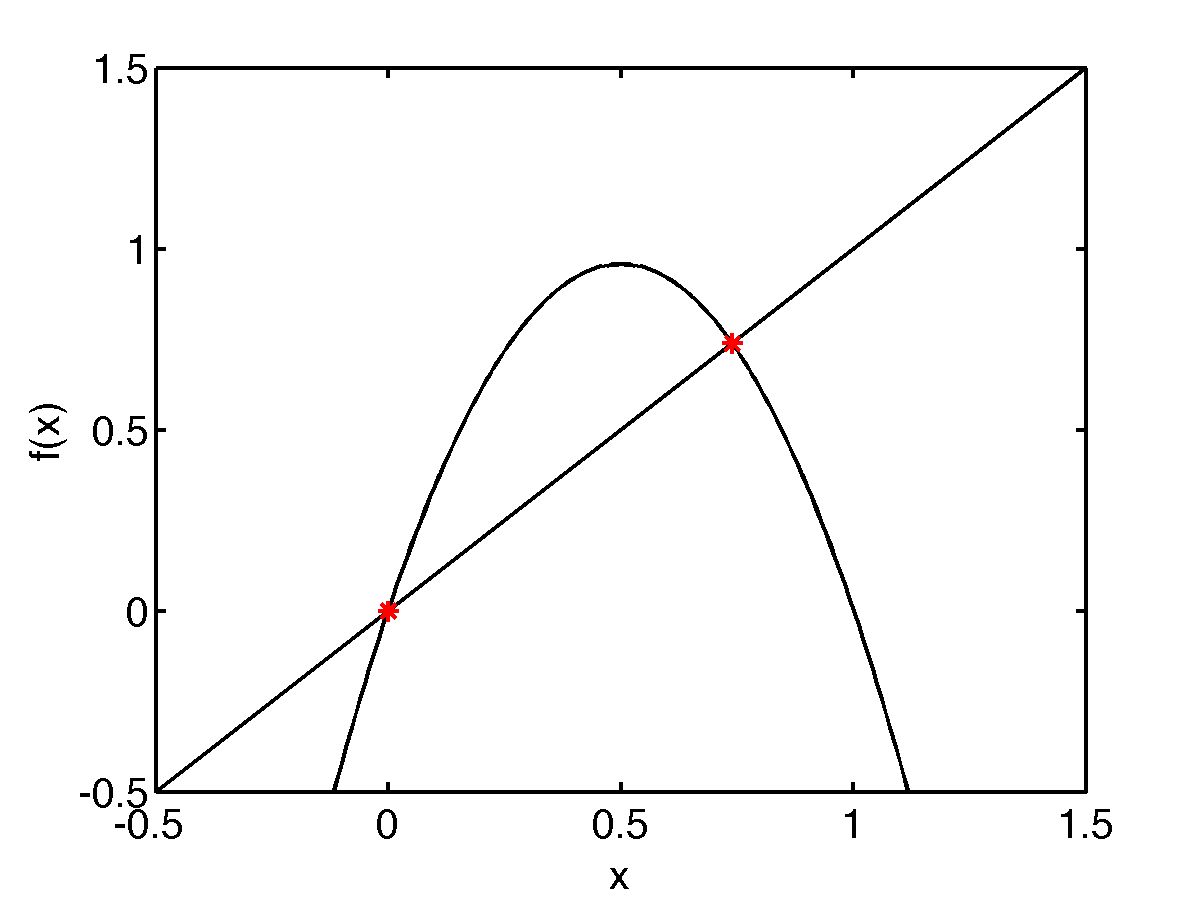
\includegraphics[width=10cm]{figs/logistic_fixed_point}
%\caption{Fixed-points of the logistic map at $\lambda=3.83$.}
%\label{figure.fixed_point}
%\end{figure}
%
%The fixed-points of the logistic map are straight-forward to solve for algebraically. The fixed-point equation for the logistic map,
%\begin{eqnarray*}
%x^* = \lambda x^* (1-x^*),
%\end{eqnarray*}
%defines a quadratic in $x^*$ possessing two solutions,
%\begin{eqnarray*}
%x^* = 0 \; \text{and} \; x^* = \frac{\lambda-1}{\lambda},
%\end{eqnarray*}
%which exist for all values of $\lambda \ne 0$. At $\lambda=0$ only the fixed-point at $x^*=0$ exists. In Figure \ref{figure.fixed_point_analytical} we plot both fixed-points as a function of $\lambda$. Notice that the non-zero fixed-point passes through a singularity at $\lambda = 0$.
%
%\begin{figure}[h]
%\centering
%\includegraphics[width=10cm]{figs/logistic_fixed_point_analytical}
%\caption{Fixed-points of the logistic map as a function of $\lambda$}
%\label{figure.fixed_point_analytical}
%\end{figure}
%
%\begin{del}
%Determine the fixed-points of the Ricker map, and plot them as a function of $\lambda$.
%\end{del} 
%
%\section*{Stability of Fixed-Points}
%
%In the previous section we showed that two fixed-points exist for all values of $\lambda$ (except $\lambda = 0$). In the orbit diagram earlier we saw that only sometimes does the sequence converge to one of these fixed-points. For example $x^*=0$ is a fixed-point for $\lambda>1$ but the orbits do not converge to it. The {\bf existence} of a fixed-point does not imply that the orbit will converge to it. A necessary (but not sufficient) condition for convergence is that the fixed-point be {\bf stable}. We will use cobweb diagrams to explore what we mean by this new term.
%
%Consider the fixed-point $x^*=0$. Certainly if we choose the initial condition $x(0) = 0$ then $x(1) = 0$, $x(2) = 0$, and so forth. This shouldn't be surprising as this is the definition of a fixed-point - a value that is mapped to itself after one iteration. What if we start close to, but not exactly equal to zero? In Figure \ref{} we show the cobweb diagram for $\lambda = 0.5$, and $\lambda = 2$. In the first case, the orbit is {\bf attracted} to the fixed-point at zero and will eventually converge to it. In the second case, the orbit is {\bf repelled} from the fixed-point at zero and eventually converges to the other fixed-point at $x^*=1$. What's the difference?
%
%The only difference between these two examples is the shape of the map itself. If we start our iterations close to the fixed-point then it's the shape of the map close to the fixed-point that matters. In particular, notice that the slope of the function at $x=0$ is less than one in the first example, but greater than one in the second example. The slope of a function is given by the derivative, and it appears then that if the slope of the function at the fixed-point is greater than 1 then an orbit which begins close to the fixed-point is repelled from it, and the fixed-point is termed {\bf unstable}.
%
%We've also seen evidence that if the derivative of the map at the fixed-point is less than 1 then the orbit will converge to the fixed-point. This does not always hold however, as we see in the cobweb diagram for $\lambda = 4$. In this case, the slope of the function at the non-zero fixed-point is $-2$, and the fixed-point is repelling. This leads us to the following conjecture
%
%\begin{con}
%A fixed-point $x^*$ is stable if $|f'(x^*)| < 1$ and unstable if $|f'(x^*)| > 1$.  
%\end{con}
%
%The stability of both fixed-points of the logistic map can now be determined by appealing to this conjecture. The derivative of the logistic map is
%\begin{eqnarray*}
%f'(x) = \lambda (1 - 2x).
%\end{eqnarray*}
%Consider the fixed-point $x^* = 0$. In this case
%\begin{eqnarray*}
%f'(x^*) = \lambda,
%\end{eqnarray*}
%and the fixed-point at the origin is stable if $-1 < \lambda < 1$, and unstable if $|\lambda| > 1$. This is consistent with the orbit diagram in Figure \ref{}. Now consider the fixed-point at $x^* = \frac{\lambda-1}{\lambda}$. In this case
%\begin{eqnarray*}
%f'(x^*) = -\lambda + 2
%\end{eqnarray*}
%and the fixed-point is stable if $1 < \lambda < 3$, which is again consistent with the orbit diagram.
%
%\begin{del}
%Determine the stability of the fixed-points of the Ricker map.
%\end{del} 
%
%As mentioned earlier, the stability of a fixed-point is necessary but not sufficient for orbits to converge to it. Stability only guarantees that an orbit which begins close to the fixed-point will converge to it. The set of initial conditions that converge to a stable fixed-point is known as the {\bf basin of attraction} of the fixed-point. 
%
%\section*{Basin of Attraction}
%
%If a fixed-point is stable then its basin of attraction is guaranteed to be non-empty, but it could be very small - on the other hand it could be the whole number line. Consider the fixed-point $x^* = 0.5$ at $\lambda = 2$. We just found that this fixed-point is stable. What is its basin of attraction? 
%
%We saw earlier that if we choose $x(0) > 1$ or $x(0) < 0$  then the orbit diverges to $-\infty$. If we choose $x(0) = 1$ or $x(0) = 0$, then $x(1) = 0$ which is a fixed-point. If we choose $x(0)$ just less than 1 then $x(1)$ is just greater than zero. However, the fixed-point at the origin is unstable so the orbit will move away from it. We also know from earlier that the orbit is bounded to the unit interval so can we assume that it will eventually converge to the fixed-point at $0.5$? Almost, but not quite, because the orbit could land on a periodic orbit instead (if one exists). Still, we can say that the basin of attraction for the fixed-point at $0.5$ is $(0,1)$ except for points that are eventually periodic.
%
%\begin{del}
%What is the basin of attraction of the fixed-points of the Ricker map?
%\end{del}
%
%\section*{Periodic Orbits}
%A {\bf period-k orbit} of a map is defined as those points which are mapped to themselves after $k$ iterations. A fixed point is therefore a period-1 orbit. Note that this implies that there are $k$ periodic points associated with a given period-k orbit. For example, a period-2 orbit has two period-2 points, $p$ and $q$, which satisfy
%\begin{eqnarray*}
%q &=& f(p), \\
%p &=& f(q).
%\end{eqnarray*}
%The orbit, starting with initial condition $p$, would be $\{p, q, p, q, p, q, \ldots\}$. 
%
%A cobweb diagram is a useful way of looking for periodic-orbits qualitatively. For example, a period-2 orbit would "look" like a rectangle as shown in Figure () for the logistic map at $\lambda = 3.5$. This demonstrates that a period-2 orbit exists at this value of $\lambda$. However, if you try to draw a rectangle for $\lambda = 2$ you will quickly discover that it cannot be done.
%
%\begin{del}
%For which values of $\lambda$ of the logistic map can you draw a rectangle and therefore define a period-2 orbit? How about a period-3 orbit, which is an irregular hexagon? What about the Ricker map?
%\end{del}
%
%Alternatively, we can define a period-2 orbit as those points which satisfy
%\begin{eqnarray*}
%p = f(f(p))
%\end{eqnarray*}
%The period-2 points are therefore fixed points of the {\bf second-return} map, and we can use the tools previously discussed for fixed-points. For example, the fixed-points of the second-return of the logistic map are defined by
%\begin{eqnarray*}
%p = \lambda (\lambda p(1-p))(1 - \lambda p(1-p))
%\end{eqnarray*}
%which (when you distribute the terms) looks like a rather nasty fourth degree polynomial in $p$. The fundamental theorem of algebra guarantees that there exists exactly four solutions (possibly complex) counting multiplicities. However, we already know two of them because {\bf fixed-points of the first-return map are fixed-points of the second-return map too}. Do you remember in school when you learned how to divide polynomials, and you were wondering why you should care? Well, now we can factor out two roots from this fourth-degree polynomial using synthetic division and reduce it to a second-order polynomial whose solutions we can write down. Recall that the fixed-points are $p=0$ and $p = \frac{\lambda - 1}{\lambda}$ so we factor out
%\begin{eqnarray*}
%(p-0)(p-\frac{\lambda-1}{\lambda})
%\end{eqnarray*}
%from the fourth-degree polynomial and reduce it to the second-order polynomial
%\begin{eqnarray*}
%\end{eqnarray*}
%which has real solutions if
%\begin{eqnarray*}
%\end{eqnarray*}
%Period-2 points of the logistic map therefore exist when
%\begin{eqnarray*}
%\end{eqnarray*}
%which is at least consistent with the orbit diagram from earlier.
%
%Unfortunately, this algebraic approach is only possible for some maps. The logistic map is a good example because it is a polynomial map. The Ricker map on the other hand is a transcendental map and this approach is likely to fail (try it and see what happens!). We therefore need to adopt one of the other approaches discussed earlier. In Figure () we plot the second-return of the logistic map for different values of $\lambda$. The intersections of the map with the unity line define the fixed-points and the period-2 points. For $\lambda = 2$ only the fixed-points at $p=0$ and $p=1$ exist. At $\lambda = 4$ however both the fixed-points $p=0$ and $p=3/4$ and two period-2 points exist - their values are $p=$ and $p=$ which agrees with our earlier algebraic work. As we increase $\lambda$ from 2 to 4, notice how the map changes and that the period-2 points suddenly appear at $\lambda = 3$. 
%
%\begin{del}
%Write a MATLAB script that plots the second-return Ricker map and find the critical value of $\lambda$ at which the period-2 orbit springs into existence.
%\end{del}
%
%Is it a coincidence that the period-2 orbit of the logistic map 'appears' at $\lambda = 3$ which is the value of $\lambda$ at which the first-derivative of the map evaluated at the non-zero fixed-point is -1? Is this true for the Ricker map too?



%
% 
%
%
%\bibliography{nldc_book}
%\bibliographystyle{plainnat}
%
%\end{document}
%
%
%The period-2 points are therefore fixed points of the {\bf second-return} map $f^2$.
%\begin{quote}
%Graphically determine the period-2 orbits of the logistic map and the tent map for any value of the control parameter and then find them analytically.Confirm your findings using your graphical iteration program.
%\end{quote}
%\begin{quote}
%Graphically determine the period-3 orbits of the tent map for any value of the control parameter and then find them analytically.
%\end{quote}
%
%\subsection{Stability of Fixed Points and Periodic Orbits}
%Consider a fixed point $p$ which satisfies $p=f(p)$. If all points sufficiently close to $p$ are attracted to $p$ then $p$ is called a {\bf sink} or an attracting fixed point. If all points sufficiently close to $p$ are repelled from $p$, then $p$ is called a {\bf source} or a repelling fixed point. The {\bf Linear Stability Theorem} gives conditions for when a fixed point is a {\bf sink} or a {\bf source}:
%\begin{quote}
%If $|f '(p)| < 1$, then $p$ is a sink.
%\end{quote}
%\begin{quote}
%If $|f '(p)| > 1$, then $p$ is a source.
%\end{quote}
%\begin{quote}
%Determine the stability of the fixed points of the logistic map for any value of $\lambda$ and of the tent map for any value of $a$.
%\end{quote}
%Periodic orbits can be treated in much the same way by recalling, for example, that a period-2 point is a fixed-point of the second-return map $f^2$. Using the chain rule we see that
%\begin{eqnarray*}
%\left. \frac{d}{dx} f(f(x)) \right|_{x=p} = f '(f(p)) f '(p) = f '(q) f '(p)
%\end{eqnarray*}
%which implies that the stability of the two period-2 points is identical.
%\begin{quote}
%Determine the stability of the period-2 orbit of the logistic map and the period-2 orbit of the tent map.
%\end{quote}
%\begin{quote}
%Determine the stability of every period-k orbit of the tent map.
%\end{quote}
%
%Rather than rely on algebraic solutions we will now determine the fixed-points of the logistic map numerically. A reasonable approximation can be made by laying down a large number of search points on a given search interval, computing one iteration of the map, and finding the points which have returned close to themselves. In Figure (\ref{figure.logistic_fixed_point_numerical}) we plot the numerically determined fixed-points of the logistic map. At each value of $\lambda$ we lay down 1000 equally-spaced points on $[-1,2]$ and find the points which move by less than $10^{-3}$ after one iteration. Hopefully you recognise the fixed-point $x^*=0$ and the family of fixed-points defined by $x^*=(\lambda-1)/\lambda$ which passes through a singularity at $\lambda=0$ as expected. In later sections we will improve on this brute-force approach and determine the fixed-points with greater accuracy. It's also worth pointing out that the existence of a fixed-point does not imply that the orbit will converge to it. For example $x=0$ is a fixed-point for $\lambda>1$ but the orbits do not converge to it.
%
%\begin{figure}[h]
%\centering
%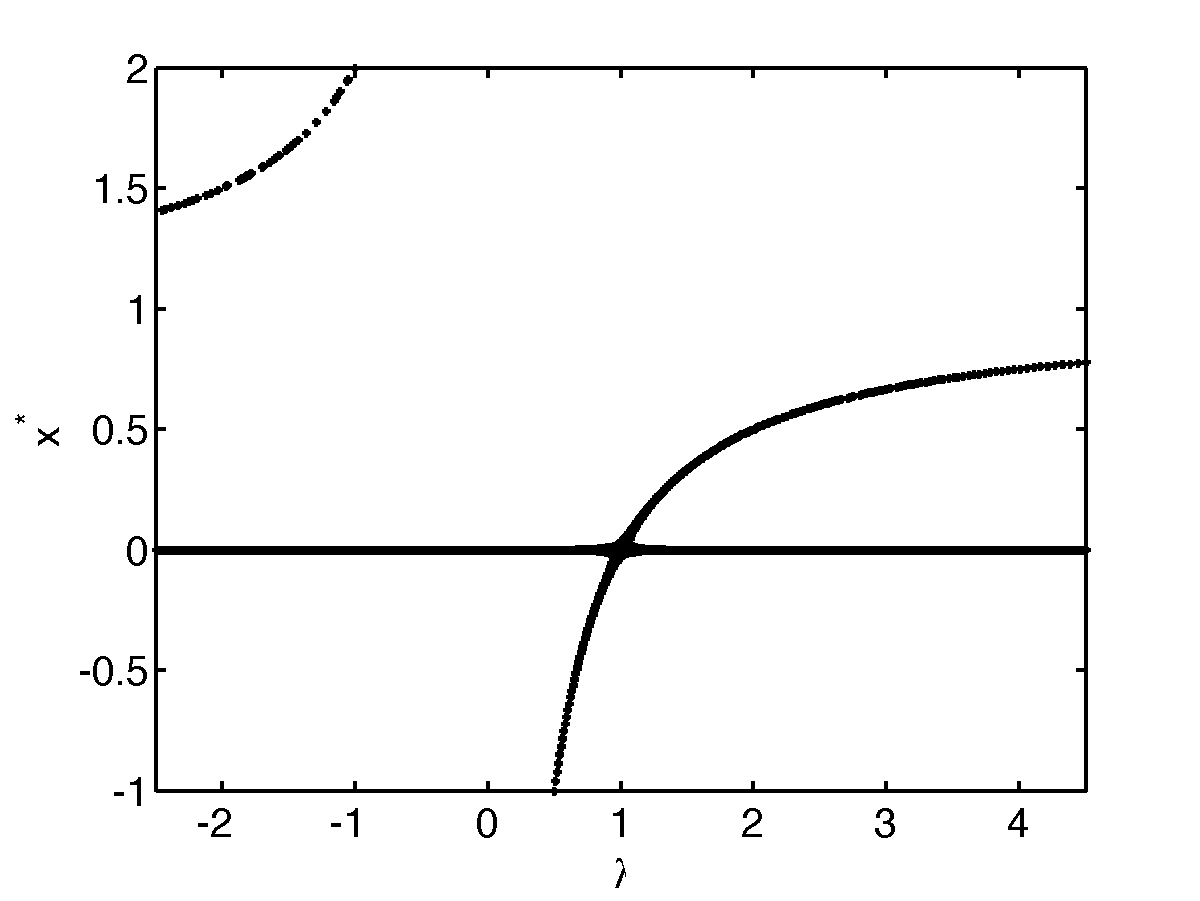
\includegraphics[width=10cm]{figs/logistic_fixed_point_numerical}
%\caption{Numerically computed fixed-points of the logistic map for various values of $\lambda$.}
%\label{figure.logistic_fixed_point_numerical}
%\end{figure}
%
%\begin{del}
%Write a computer program to numerically compute the fixed-points of the Ricker map for various values of the control parameter.
%\end{del}
%
%
%\subsection{Fixed Points}
%\begin{quote}
%Graphically determine the fixed point(s) of the logistic map and the tent map for any value of the control parameter and then find them analytically for any value of $\lambda$ and $a$.
%\end{quote}
%
%\subsection{Periodic Orbits}
%A {\bf period-k orbit} of a 1D map is defined as those points which are mapped to themselves after $k$ iterations. A fixed point is therefore a period-1 orbit. Note that this implies that there are $k$ periodic points associated with a given period-k orbit. For example, a period-2 orbit has two period-2 points, $p$ and $q$, which satisfy
%\begin{eqnarray*}
%q &=& f(p), \\
%p &=& f(q).
%\end{eqnarray*}
%The orbit, starting with initial condition $p$, would be $\{p, q, p, q, p, q, \ldots\}$. Alternatively, we can define a period-2 orbit as those points which satisfy
%\begin{eqnarray*}
%p = f(f(p)) = f^2(p)
%\end{eqnarray*}
%The period-2 points are therefore fixed points of the {\bf second-return} map $f^2$.
%\begin{quote}
%Graphically determine the period-2 orbits of the logistic map and the tent map for any value of the control parameter and then find them analytically.Confirm your findings using your graphical iteration program.
%\end{quote}
%\begin{quote}
%Graphically determine the period-3 orbits of the tent map for any value of the control parameter and then find them analytically.
%\end{quote}
%
%\subsection{Stability of Fixed Points and Periodic Orbits}
%Consider a fixed point $p$ which satisfies $p=f(p)$. If all points sufficiently close to $p$ are attracted to $p$ then $p$ is called a {\bf sink} or an attracting fixed point. If all points sufficiently close to $p$ are repelled from $p$, then $p$ is called a {\bf source} or a repelling fixed point. The {\bf Linear Stability Theorem} gives conditions for when a fixed point is a {\bf sink} or a {\bf source}:
%\begin{quote}
%If $|f '(p)| < 1$, then $p$ is a sink.
%\end{quote}
%\begin{quote}
%If $|f '(p)| > 1$, then $p$ is a source.
%\end{quote}
%\begin{quote}
%Determine the stability of the fixed points of the logistic map for any value of $\lambda$ and of the tent map for any value of $a$.
%\end{quote}
%Periodic orbits can be treated in much the same way by recalling, for example, that a period-2 point is a fixed-point of the second-return map $f^2$. Using the chain rule we see that
%\begin{eqnarray*}
%\left. \frac{d}{dx} f(f(x)) \right|_{x=p} = f '(f(p)) f '(p) = f '(q) f '(p)
%\end{eqnarray*}
%which implies that the stability of the two period-2 points is identical.
%\begin{quote}
%Determine the stability of the period-2 orbit of the logistic map and the period-2 orbit of the tent map.
%\end{quote}
%\begin{quote}
%Determine the stability of every period-k orbit of the tent map.
%\end{quote}
%
%\subsection{Sensitive Dependence}
%We have already discovered that the dynamics of the logistic map for $\lambda=4$ and of the tent map for $a=2$ are ``crazy''. The orbits seem to wander around forever, never reaching a fixed point nor a periodic orbit. In addition, two points which are close to begin with eventually move apart. The orbit seems to depend sensitively on the initial conditions.
%\begin{quote}
%Write a program that computes the number of iterations it takes for two points separated by $10^{-p}$ to separate by at least $1/2$. Do this for both the logistic map $\lambda = 4$ and the tent map $a=2$. Choose the first point at random on the unit interval. Plot your results as a function of the exponent $p$. 
%\end{quote}
%
%\subsection{Itineraries}
%The logisitic map and the tent map are very similar - in particular they are both symmetric about the $x=1/2$ point. This suggests that we could label an initial condition as belonging to the {\bf L}eft-half of the unit interval or the {\bf R}ight-half of the unit interval. What then is the set of points on the unit interval that begin in the {\bf L}eft-half and after one iteration are again in the {\bf L}eft-half. We might label such a set of points as $LL$? For the tent map ($a=2$) the set of points that defines $LL$ is given by $[0,1/4)$. The set of points that defines $RL$ is given by $[3/4,1]$.
%
%\begin{quote}
%Find the set of points that defines $LR$ and $RL$ for the tent map with $a=2$. Repeat this entire exercise for the logistic map for $\lambda = 4$.
%\end{quote}
%
%\begin{quote}
%How many different itineraries are there that consists of three symbols? Do they come in a predictable order on the unit interval? What are they for the tent map? What are they for the logistic map? Can you compute then in general for an orbit consisting of $k$ symbols?
%\end{quote}
%
%The itineraries tell us quite a bit about the dynamics of the tent map and the logistic map. For example, consider the tent map and the set of points that defines an itinerary $S_1 S_2 \ldots S_k$ for large $k$. This interval has sub-intervals $S_1 S_2 \ldots S_k L L$, $S_1 S_2 \ldots S_k L R$, $S_1 S_2 \ldots S_k R R$, and $S_1 S_2 \ldots S_k R L$. If we choose a point in the subinterval ending in $LL$ and a point in the subinterval ending in $RL$ then after $k-1$ iteration, these initial conditions (which were initially less than $2^{-k}$ apart) are now more than $1/2$ apart!
%
%\subsection{Lyapunov Number}
%The findings on sensitive dependence and itineraries can be nicely summarized by defining the Lyapunov number. A period-2 orbit separates close initial conditions by a factor $\sqrt{|f'(p)||f'(q)|}$ after each iteration. A period-k orbit would separate close initial conditions by a factor of
%\begin{equation}
%\left(|f'(p_1)||f'(p_2)| \ldots |f'(p_k)|\right)^{1/k}
%\end{equation}
%This naturally motivates the definition of a stretching number or Lyapunov number for a given orbit ${p_0, p_1, p_2, \ldots, p_n}$ as
%\begin{equation}
%L = \lim_{n \rightarrow \infty} \left(|f'(p_1)||f'(p_2)| \ldots |f'(p_n)|\right)^{1/n}
%\end{equation}
%
%\begin{quote}
%Show that the Lyapunov number for the tent map with $a=2$ is $2$. Compute the Lyapunov number for the logistic map as a function of $\lambda$.
%\end{quote}
%
%\subsection{Chaotic Orbit}
%An orbit is chaotic if it is not eventually periodic and if the Lyapunov number is $> 1$.
%
%\clearpage
%
%
%\end{document}
%
% For a given $t \in T$ a map $\phi^t$ is defined in the state space $X$,
%\begin{eqnarray}
%\phi^t: X \rightarrow X,
%\end{eqnarray}
%which transforms an initial state $\mathbf{x}_0 \in X$ into some state $\mathbf{x}_t \in X$ at time $t$,
%\begin{eqnarray}
%\mathbf{x}_t = \phi^t \mathbf{x}_0.
%\end{eqnarray}
%The map $\phi^t$ is the evolution operator of the dynamical system and can usually be computed only approximately. 
%
%The evolution operators discussed in this book have two properties that reflect the deterministic behavior of the dynamical system. The first property,
%\begin{eqnarray}
%\phi^0 = \mbox{identity},
%\label{eq:identity}
%\end{eqnarray}
%rules out spontaneous changes in state, i.e. $\phi^0 \mathbf{x} = \mathbf{x}$. The second property,
%\begin{eqnarray}
%\phi^{t+s} = \phi^t  \phi^s,
%\label{eq:compose}
%\end{eqnarray} 
%means that the rules governing the evolution of the dynamical system do not change in time, i.e. $\phi^{t+s} \mathbf{x} = \phi^t(\phi^s \mathbf{x})$. A state which evolves $t+s$ units in time arrives at the same state as one which evolves $s$ units of time and then $t$ units of time. The formal definition of a dynamical system can now be given:
%
%\begin{quote}
%A dynamical system is a triple $\{T,X,\phi^t\}$, where $T$ is a time set, $X$ is a state space, and $\phi^t : X \rightarrow X$ is a family of evolution operators parameterized by $t \in T$ and satisfying properties (\ref{eq:identity}) and (\ref{eq:compose}).
%\end{quote}
%
%\section*{What are these notes about?}
%
%Models of the natural world are often deterministic. The future and past states of a deterministic system can be predicted by knowing the present state of the system and the deterministic laws that govern their evolution. If you are a student of classical physics, or of most engineering disciplines, then the models that you have been exposed to, and been expected to use, are probably deterministic. Stochastic models on the other hand involve an element of randomness, but we will not consider such models in this book.
%
%A dynamical system is in some sense a mathematical representation of a deterministic model and is defined by its possible states and a law for the evolution of the state in time. The possible states of a dynamical system are defined by the points of some set $X$, which is called the state space of the system. Typically, but not always, the state space is finite, e.g. $X = \mathbf{R}$ or $X = \mathbf{S} \times \mathbf{R}$. Infinite-dimensional state spaces are possible, e.g. $X = $ set of integrable functions, but we will not consider this type of dynamical system in this book.
%
%A dynamical system evolves over time $t \in T$, where $T$ is a number set. These notes deal with both discrete- and continuous-time dynamical systems. A discrete-time dynamical system is defined over discrete (integer) time $T=\mathbf{Z}$. A continuous-time dynamical system is defined over continuous (real) time $T=\mathbf{R}$. In either case, an evolution law determines the state $\mathbf{x}(t)$ of the system at time $t$ given the initial state $\mathbf{x}(0)$.
%
%\begin{figure}[h]
%\includegraphics{figs/dynamicalsystem}
%\caption{A dynamical system is defined by a set of points in a state space and an evolution law over time (picture of state space and evolution operator).}
%\end{figure}
%
%\section*{How are these notes organized?}
%
%These notes are divided into two main parts. The first part is devoted to the most common example of a discrete-time evolution law, namely a difference equation,
%\begin{eqnarray}
%\mathbf{x}(t+1) = \mathbf{F}(\mathbf{x}(t)) \hspace{1cm} t = 0, 1, 2, \ldots,
%\label{eq.difference}
%\end{eqnarray}
%which takes an initial condition $\mathbf{x}(0) \in \mathbf{R}^N$ and generates a sequence $\mathbf{x}(0), \mathbf{x}(1), \mathbf{x}(2), \ldots$ by repeated iteration of the function $\mathbf{F}: \mathbf{R}^N \rightarrow \mathbf{R}^N$. The solution of Eq. (\ref{eq.difference}) then is the sequence $\{\mathbf{x}\}$. In these notes we are primarily interested in the long-term behavior of the system, i.e. the behaviour of the sequence as $t \rightarrow \infty$. 
%
%The second part of the notes is focused on ordinary differential equation (ODEs), which are the most common example of a continuous-time dynamical system. An $N$th-order ODE,
%\begin{eqnarray}
%\dot{\mathbf{x}} = \mathbf{F}(\mathbf{x}),
%\label{eq.differential}
%\end{eqnarray}
%takes an initial condition $\mathbf{x}(0) \in \mathbf{R}^N$ and generates a function $\mathbf{x}(t)$ whose derivative is $\mathbf{F}$ for all $t \ge 0$. The solution of Eq. (\ref{eq.differential}) is the function $\mathbf{x}$, although it may only be defined for finite $t$. Again we are primarily interested in the behaviour of the solution as $t \rightarrow \infty$. 
%
%These notes are organized into two halves and the material in each half of the notes is organized into two case studies. The opening case study is devoted to first-order difference equations ($N=1$), while the second is focused on difference equations of order 2 or greater ($N \ge 2$). The third case study examines the dynamics of a single first-order ODE, while the fourth and last case study concerns ODE's in the plane ($N=2$). We will end by previewing the results for ODE's of order 3 or greater ($N \ge 3$). At the end of each case study there are suggestions for projects that the interested reader might wish to pursue.
%
%\begin{figure}[h]
%\includegraphics{figs/square}
%\caption{These notes are organized around discrete- and continuous-time dynamical systems in both low and high dimensions. (picture of square broken into 4 pieces, each with a representative image (period-doubling, Henon or Mandelbrot, Phase plane, Lorenz)}
%\label{square}
%\end{figure}
%
%\begin{table}
%\centering
%\begin{tabular}{ccccc}
%& $\lambda$ = 2 & $\lambda$ = 3.2 & $\lambda$ = 3.83 & $\lambda$ = 3.9 \\
%x(0) & 0.2500 & 0.2500 & 0.2500 & 0.2500 \\
%x(1) & 0.3750 & 0.6000 & 0.7181 & 0.7312 \\.&
%0.4688 & 0.7680 & 0.7753 & 0.7664 \\.&
%0.4980 & 0.5702 & 0.6673 & 0.6981 \\.&
%0.5000 & 0.7842 & 0.8503 & 0.8219 \\.&
%0.5000 & 0.5415 & 0.4874 & 0.5709 \\.&
%0.5000 & 0.7945 & 0.9569 & 0.9554 \\.&
%0.5000 & 0.5225 & 0.1580 & 0.1662 \\.&
%0.5000 & 0.7984 & 0.5095 & 0.5404 \\.&
%0.5000 & 0.5151 & 0.9572 & 0.9686 \\.&
%0.5000 & 0.7993 & 0.1571 & 0.1185 \\.&
%0.5000 & 0.5134 & 0.5071 & 0.4074 \\.&
%0.5000 & 0.7994 & 0.9573 & 0.9416 \\.&
%0.5000 & 0.5131 & 0.1565 & 0.2146 \\.&
%0.5000 & 0.7995 & 0.5057 & 0.6573 \\.&
%0.5000 & 0.5131 & 0.9574 & 0.8785 \\.&
%0.5000 & 0.7995 & 0.1563 & 0.4162 \\.&
%0.5000 & 0.5130 & 0.5050 & 0.9476 \\.&
%0.5000 & 0.7995 & 0.9574 & 0.1937 \\.&
%0.5000 & 0.5130 & 0.1562 & 0.6091 \\.&
%0.5000 & 0.7995 & 0.5048 & 0.9286 \\.&
%0.5000 & 0.5130 & 0.9574 & 0.2585 \\.&
%0.5000 & 0.7995 & 0.1562 & 0.7476 \\.&
%0.5000 & 0.5130 & 0.1562 & 0.6091 \\.&
%0.5000 & 0.7995 & 0.5048 & 0.9286 \\.&
%0.5000 & 0.5130 & 0.9574 & 0.2585 \\.&
%0.5000 & 0.7995 & 0.1562 & 0.7476 \\.&
%0.5000 & 0.5130 & 0.5047 & 0.7358 \\.&
%0.5000 & 0.7995 & 0.9574 & 0.7581 \\.&
%0.5000 & 0.5130 & 0.1562 & 0.7152 \\.&
%0.5000 & 0.7995 & 0.5047 & 0.7943 \\.&
%0.5000 & 0.5130 & 0.9574 & 0.6371 \\.&
%0.5000 & 0.7995 & 0.1562 & 0.9017 \\.&
%0.5000 & 0.5130 & 0.5047 & 0.3458 \\.&
%0.5000 & 0.7995 & 0.9574 & 0.8823 \\.&
%0.5000 & 0.5130 & 0.1561 & 0.4050 \\.&
%0.5000 & 0.7995 & 0.5047 & 0.9398 \\.&
%0.5000 & 0.5130 & 0.9574 & 0.2207 \\.&
%0.5000 & 0.7995 & 0.1561 & 0.6707 \\.&
%0.5000 & 0.5130 & 0.5047 & 0.8613 \\.&
%0.5000 & 0.7995 & 0.9574 & 0.4658 \\.&
%0.5000 & 0.5130 & 0.1561 & 0.9704 \\.&
%0.5000 & 0.7995 & 0.5047 & 0.1119 \\.&
%0.5000 & 0.5130 & 0.9574 & 0.3875 \\ x(40) &
%0.5000 & 0.7995 & 0.1561 & 0.9257   
%\end{tabular}
%\caption{The first forty iterates of the logistic map for different values of the control parameter $\lambda$, but with the same initial condition $x(0) = \frac{1}{4}$. Only the first four decimal places are shown.}
%\label{table.logistic_data}
%\end{table}
%
%Of course, there are many other models one could propose, even for a single stock system.  For example, a second order model in which the birth rate depends linearly on the population might be sensible in a situation where the density of organisms controls the likelihood of conception:
%
%$$E(t+1) = E(t) + g(\frac{E(t)}{D})E(t) - dE(t)$$
%
%It is also easy to imagine situations in which birth rates or death rates depend explicitly on iteration number.  For example, a government policy might require that in every tenth year, there is an elephant cull that removes 50\% of the population:
%
%$$E(t+1) = E(t) + bE(t) - dE(t) -c(t) E(t)$$
%
%where $c(t)$ is the culling function that is, in normal years, zero, but is $0.5$ in every tenth year.
%
%
%Exercise
%
%Rabbits reproduce, as you know, like rabbits.  
%Create a model for rabbit population in a suburban setting.  Assume the following effects are present:
%\begin{itemize}
%\item Only so many gardens:  Due to suburbanites' bad experiences with rabbits nibbling on lettuce and carrots, the food supply in town is limited.
%\item Intolerant population: Whenever the population of rabbits gets too high, the townspeople get up in arms, and the local vermin control companies start targeting rabbits.  Of course, once the population drops again, the vermin control companies turn their attention back to cockroaches and mice.
%\end{itemize}
%Make a stock and flow, and a set of difference equations to capture these effects. 
%
%\subsection{Lifecycle models}
%
%Sometimes it also makes sense to keep track of different groups within a population.  Sometimes this is because of the structure of the system -- for example, in modeling progression through primary education, it might make sense to keep track of how many first graders, second graders, etc. are in the education system -- and sometimes it is due to biological features that are particular to one part of a population (e.g, human teenage males have much higher mortality rates than human adult males or human teenage females). 
%
%In a stock and flow formalism, we might assign stocks fro each of the groups within the population that we are tracking.  For example, if elephants take a certain period of time reach reproductive age, you might keep track of juvenile elephants as well as mature elephants:
%
% \centerline{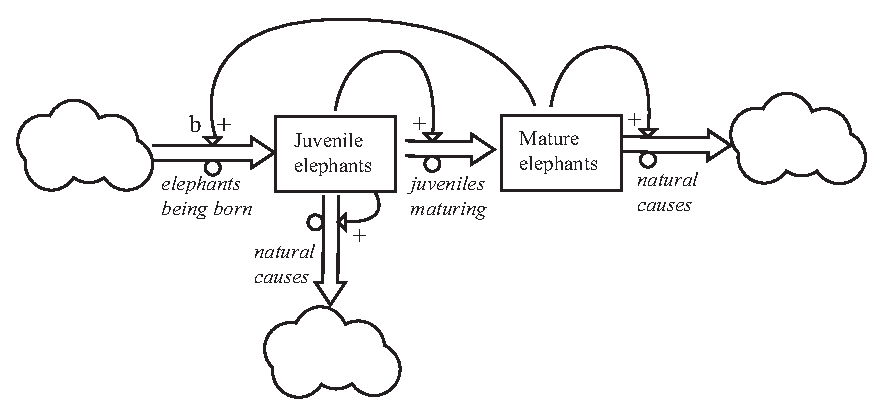
\includegraphics[height=2in]{figs/ElephantGenerationModel}}
%
%The difference equations here can be determined by looking at the diagram:
%
%\begin{eqnarray*}
%J(t+1) &=& J(t) - m J(t) - d_J J(t)+ b E(t) \\
%E(t+1) &=& E(t) + m J(t) - d_E E(t)
%\end{eqnarray*}
%
%where $J(t)$ is the number of juveniles in year $t$, $d_J$ and $d_E$ are the death rates for juveniles and adults respectively, $m$ is the maturation rate for juveniles, and $b$ is the birth rate.
%
%
%
%
